% ============================================================================
% Open-world fungal ITS embeddings.
% 11 pt article, booktabs/threeparttable tables, embedded bibliography,
% explicit VERIFY/TODO marks.
% Compile: pdflatex main.tex (twice).
%
% Tables and figures are generated from data/*.csv by
%   python3 analysis/make_tables.py
%   python3 analysis/make_figures.py
% so a number in a table can never drift from the number in the figure
% beside it. Edit the CSVs or the generators, not the .tex tables.
% ============================================================================
\documentclass[11pt]{article}
\usepackage[utf8]{inputenc}
\usepackage[T1]{fontenc}
\usepackage[a4paper,margin=1in]{geometry}
\usepackage{graphicx}
\usepackage{amsmath}
\usepackage{booktabs}
\usepackage{threeparttable}
\usepackage{authblk}
\usepackage{xcolor}
\usepackage[protrusion=true,expansion=false]{microtype}
\usepackage{url}
\usepackage{xurl}
\usepackage[hidelinks]{hyperref}
\renewcommand{\ttdefault}{cmtt}

% Line numbers for review copies: uncomment both lines.
% \usepackage{lineno}
% \linenumbers

% ---------------------------------------------------------------------------
% Draft marks. Set \draftmarksfalse to typeset a clean submission copy without
% touching the body text; every VERIFY and TODO then disappears.
% ---------------------------------------------------------------------------
\newif\ifdraftmarks
\draftmarksfalse
\definecolor{todoblue}{rgb}{0.0,0.25,0.75}
\ifdraftmarks
  \newcommand{\verify}[1]{\textcolor{red}{[VERIFY: #1]}}
  \newcommand{\todo}[1]{\textcolor{todoblue}{[TODO: #1]}}
\else
  \newcommand{\verify}[1]{}
  \newcommand{\todo}[1]{}
\fi

\renewcommand{\topfraction}{0.9}
\renewcommand{\bottomfraction}{0.7}
\renewcommand{\textfraction}{0.1}
\renewcommand{\floatpagefraction}{0.75}

% Result-forward title, scoped to the two claims this manuscript supports:
% (1) structured embeddings preserve higher-rank and cross-view taxonomy;
% (2) on a homologous ITS2 benchmark, identity remains the stronger novelty score.

% Every result number quoted in the prose is a macro generated from data/.
% generated by analysis/make_primary.py; do not edit by hand
\newcommand{\MfAUCCore}{0.756}
\newcommand{\MsAUCCore}{0.754}
\newcommand{\IdAUCCore}{0.734}
\newcommand{\MfKnownCore}{71.2\%}
\newcommand{\IdKnownCore}{83.4\%}
\newcommand{\MfFamCore}{64.8\%}
\newcommand{\IdFamCore}{84.6\%}
\newcommand{\MfOrdCore}{92.5\%}
\newcommand{\IdOrdCore}{97.0\%}
\newcommand{\MfClsCore}{97.1\%}
\newcommand{\IdClsCore}{98.7\%}
\newcommand{\DAUCCore}{+0.022}
\newcommand{\GbLoCore}{-0.069}
\newcommand{\GbHiCore}{+0.104}
\newcommand{\MfDetCore}{6.0\%}
\newcommand{\IdDetCore}{14.6\%}
\newcommand{\MfFnCore}{3.7\%}
\newcommand{\IdFnCore}{3.2\%}
\newcommand{\IdGapCore}{+0.075}
\newcommand{\MfGapCore}{+0.021}
\newcommand{\NGenCore}{183}
\newcommand{\MfAUCOne}{0.699}
\newcommand{\MsAUCOne}{0.716}
\newcommand{\IdAUCOne}{0.700}
\newcommand{\MfKnownOne}{61.6\%}
\newcommand{\IdKnownOne}{80.9\%}
\newcommand{\MfFamOne}{54.3\%}
\newcommand{\IdFamOne}{81.6\%}
\newcommand{\MfOrdOne}{84.4\%}
\newcommand{\IdOrdOne}{94.4\%}
\newcommand{\MfClsOne}{93.3\%}
\newcommand{\IdClsOne}{96.5\%}
\newcommand{\DAUCOne}{-0.001}
\newcommand{\GbLoOne}{-0.116}
\newcommand{\GbHiOne}{+0.097}
\newcommand{\MfDetOne}{5.5\%}
\newcommand{\IdDetOne}{8.4\%}
\newcommand{\MfFnOne}{4.9\%}
\newcommand{\IdFnOne}{4.0\%}
\newcommand{\IdGapOne}{+0.107}
\newcommand{\MfGapOne}{+0.041}
\newcommand{\NGenOne}{184}
\newcommand{\MfAUCTwo}{0.740}
\newcommand{\MsAUCTwo}{0.763}
\newcommand{\IdAUCTwo}{0.735}
\newcommand{\MfKnownTwo}{66.2\%}
\newcommand{\IdKnownTwo}{80.8\%}
\newcommand{\MfFamTwo}{53.8\%}
\newcommand{\IdFamTwo}{80.0\%}
\newcommand{\MfOrdTwo}{81.7\%}
\newcommand{\IdOrdTwo}{95.6\%}
\newcommand{\MfClsTwo}{93.2\%}
\newcommand{\IdClsTwo}{97.5\%}
\newcommand{\DAUCTwo}{+0.005}
\newcommand{\GbLoTwo}{-0.069}
\newcommand{\GbHiTwo}{+0.068}
\newcommand{\MfDetTwo}{9.6\%}
\newcommand{\IdDetTwo}{15.0\%}
\newcommand{\MfFnTwo}{4.3\%}
\newcommand{\IdFnTwo}{3.3\%}
\newcommand{\IdGapTwo}{+0.044}
\newcommand{\MfGapTwo}{+0.014}
\newcommand{\NGenTwo}{183}
\newcommand{\XIdKnownOne}{79.8\%}
\newcommand{\XIdFamOne}{70.9\%}
\newcommand{\XIdAUCOne}{0.801}
\newcommand{\XMKnownOne}{32.9\%}
\newcommand{\XMFamOne}{30.0\%}
\newcommand{\XMAUCOne}{0.581}
\newcommand{\XIdKnownTwo}{78.5\%}
\newcommand{\XIdFamTwo}{69.8\%}
\newcommand{\XIdAUCTwo}{0.779}
\newcommand{\XMKnownTwo}{24.2\%}
\newcommand{\XMFamTwo}{20.6\%}
\newcommand{\XMAUCTwo}{0.616}
\newcommand{\AudLgoPct}{62.0\%}
\newcommand{\AudLsoPct}{37.1\%}
\newcommand{\AudAllPct}{50.7\%}
\newcommand{\AudAllImpPct}{48.3\%}
\newcommand{\AudLgoGain}{2.93}
\newcommand{\AudLsoGain}{1.30}
\newcommand{\CovNoneFam}{53.7\%}
\newcommand{\CovNoneCls}{64.9\%}
\newcommand{\CovEightFam}{84.6\%}
\newcommand{\CovEightCls}{98.7\%}


% Result-forward and scoped to what the corrected evaluation supports.
% Alternative: "Leakage, search heuristics and batch padding decide
% learned-versus-alignment comparisons for open-world fungal ITS".
\title{\textbf{A learned fungal ITS embedding does not outperform correctly
configured alignment in open-world evaluation}}
\author[1]{Aaron O'Brien\thanks{Corresponding author: aaron.obrien@unab.cl}}
\author[2]{Auguste Gardette}
\affil[1]{Centro de Biotecnolog\'ia de Sistemas, Universidad Andr\'es Bello, Santiago, Chile}
\affil[2]{IRD, Sorbonne University, UMMISCO, 4 place Jussieu, Paris, France}
\date{}




\begin{document}
\maketitle

\begin{abstract}
\noindent
1.~Learned sequence embeddings are increasingly proposed for fungal ITS
classification and novelty detection, but are usually evaluated against weaker
versions of themselves or default-configured alignment, by AUROC alone, and with
queries treated as independent. We asked whether a purpose-trained encoder
outperforms percent identity when both score identical queries under a
firewalled open-world design, and which evaluation choices decide the answer.

\noindent
2.~From the UNITE release of 19 February 2025 we built ITS-core, ITS1 and ITS2
views and a genus-separated split with sealed calibration and test partitions. A
convolutional encoder trained with genus-proxy, cross-view, hierarchical and
episodic objectives was frozen and hash-sealed before test data were opened. We
compared it with exhaustive, coverage-filtered VSEARCH identity on the same
queries and references using genus-clustered paired intervals, and logged every
post-opening correction before computing corrected metrics.

\noindent
3.~Three evaluation choices changed the comparison. Default VSEARCH heuristics
returned a lower-identity hit than exhaustive search for \AudAllImpPct{} of
benchmark queries; without a coverage filter, identity placed only
\CovNoneCls{} of novel ITS-core queries in the correct class, against
\CovEightCls{} with it, because the conserved 5.8S let partial alignments win;
and the encoder's embeddings depended on inference batching. Once corrected,
identity exceeded the encoder in known-genus accuracy and novel-family placement
at every view (family \IdFamTwo{} to \IdFamCore{} against \MfFamTwo{} to
\MfFamCore{}) and detected more novel genera at a lower false-novelty rate. The
encoder's novelty AUROC was within $0.023$ of identity's, and no genus-clustered
interval excluded zero. Identity's own development-to-test gap exceeded the
encoder's, so that gap reflects partition composition rather than selection. Of
the genera held out by a historical benchmark, $85\%$ had been present in
training; on a leakage-safe version, identity's AUROC advantage was $0.065$,
with a genus-clustered interval excluding zero.

\noindent
4.~Correctly configured alignment matched or exceeded the learned embedding
throughout. The decisive results came from the evaluation, not the
representation: baseline configuration, batch invariance, genus-level
uncertainty, a parameter-free control for selection and a leakage audit each
changed a conclusion, and each is inexpensive to apply to any learned barcode
method.

\vspace{0.6em}
\noindent
\textbf{Keywords.} benchmarking; conformal prediction; data leakage; fungal ITS;
metabarcoding; novelty detection; reproducibility; VSEARCH.
\end{abstract}
% ============================================================================
\section{Introduction}
% ============================================================================
Fungal metabarcoding routinely returns sequences whose closest named relative
is distant and whose genus is absent from every reference collection
\cite{nilsson2019unite}. A method deployed on such data has two jobs: to decide
whether a query is novel enough to withhold a genus assignment, and to place it
as precisely as the reference allows. Learned sequence embeddings are an
attractive answer to both, because they promise a single similarity space in
which unseen genera sit near their relatives and in which different barcode
views become comparable
\cite{badirli2021zeroshot,badirli2023classifying,romeijn2024mycoai}.

How such methods are evaluated matters as much as how they are built. Four
habits are common. Learned models are compared chiefly with weaker variants of
themselves, so an ablation ladder can show steady improvement without saying
whether any rung beats a method practitioners already use. When an alignment
baseline is included it is usually run with default settings. Novelty is
summarised by AUROC, a whole-curve statistic, rather than by the operating
points at which a user would actually flag sequences. And uncertainty is
computed over queries as if they were independent, although queries from one
genus share most of their information. A recent systematic comparison of
classifiers for unknown barcodes, including fungal ITS, found composition-based
classifiers strongest and showed that apparent under-classification by
alignment often reflected threshold stringency rather than genuine novelty
\cite{orsholm2026unseen}; baseline configuration, in other words, can decide the
result.

We built a purpose-trained ITS encoder under a deliberately strict design: a
genus-separated split, a controlled ladder that adds one training objective at a
time, a hash-sealed freeze before calibration and test data were opened, and
split-conformal calibration of the novelty decision \cite{obrien2026flag}. The
sealed evaluation supported a positive claim about higher-rank placement and
cross-view retrieval. It did not include a non-learned baseline on the same
split. Adding one, and examining the evaluation that produced the claim, is the
subject of this paper.

The contribution is therefore an evaluation protocol with the encoder as its
worked example. We report five checks, each of which changed a conclusion here:
auditing the alignment baseline's search configuration; testing whether
embeddings are invariant to inference batching; computing paired uncertainty at
the genus rather than the query level; separating selection optimism from
partition composition with a parameter-free control; and auditing a benchmark
for training-set leakage before scoring it. Under the corrected evaluation, a
correctly configured alignment baseline matched or exceeded the learned
embedding on every comparison we could make.
\section{Methods}
% ============================================================================
\subsection{UNITE collection and ITS views}
We used the UNITE dynamic general release dated 19 February 2025
\cite{nilsson2019unite,unite2025release}. The source FASTA contained $102{,}137$
records. ITSx was run on the standard trimmed file
(\texttt{sh\_general\_release\_dynamic\_19.02.2025.fasta}) rather than its
\texttt{\_dev} variant, which holds the same records; the input lengths ITSx
recorded matched the trimmed file for 500 of 500 sampled records and the
\texttt{\_dev} file for 323. ITS regions were extracted with ITSx \cite{bengtsson2013itsx}. The
historical ITS2 collection used by the companion novelty workflow contains
$99{,}808$ sequences; a fresh extraction recovered $99{,}862$. Every historical
record was contained in the fresh extraction, so the difference is 54 additional
calls rather than any loss of historical sequences.

Three views were retained where annotated: ITS1, ITS2, and \emph{ITS-core}, the
contiguous ITS1--5.8S--ITS2 span. Exact sequence hashes identified 301
view-level groups in which an identical ITS1 or ITS2 sequence carried more than
one genus label. Rather than discard the whole source record, we masked only the
conflicting view: 393 ITS1 views and 338 ITS2 views. No cross-genus exact
conflict was detected for ITS-core. Requiring a named family and genus left
$67{,}406$ records for open-world splitting (Table~\ref{tab:dataset}).

\begin{table}[htbp]\centering
\begin{threeparttable}
\caption{Source collection and open-world partitioning. \emph{Records} counts source records after taxonomic filtering; the three right-hand columns give how many of those records carry each barcode view and are therefore the denominators for the per-view results in Tables~\ref{tab:headtohead}--\ref{tab:operating}.}
\label{tab:dataset}
\small
\setlength{\tabcolsep}{5pt}
\begin{tabular}{lrrrr}
\toprule
 & & \multicolumn{3}{c}{records carrying the view} \\
\cmidrule(l){3-5}
item & records & ITS-core & ITS1 & ITS2 \\
\midrule
\multicolumn{5}{l}{\emph{Source collection}} \\
\quad UNITE dynamic release (19 Feb 2025) & 102,137 & --- & --- & --- \\
\quad historical ITS2 pool & 99,808 & --- & --- & --- \\
\quad fresh ITS2 extraction & 99,862 & --- & --- & --- \\
\quad named family and genus & 67,406 & --- & --- & --- \\
\addlinespace
\multicolumn{5}{l}{\emph{Open-world partitions}} \\
\quad TRAIN\_REF & 46,453 & 46,151 & 46,342 & 46,076 \\
\quad DEV\_KNOWN & 1,528 & 1,515 & 1,527 & 1,515 \\
\quad DEV\_NOVEL & 8,698 & 8,659 & 8,682 & 8,642 \\
\quad CAL\_KNOWN & 1,505 & 1,494 & 1,501 & 1,493 \\
\quad TEST\_KNOWN & 1,484 & 1,467 & 1,477 & 1,463 \\
\quad TEST\_NOVEL & 7,738 & 7,718 & 7,702 & 7,671 \\
\addlinespace
\quad total partitioned & 67,406 & & & \\
\bottomrule
\end{tabular}
\begin{tablenotes}\footnotesize
\item Exact cross-genus sequence conflicts were masked at the level of the individual view rather than by deleting the source record: 393 ITS1 and 338 ITS2 views across 301 conflict groups. No ITS-core conflict was detected.
\item The six partitions sum exactly to the named-family-and-genus total.
\end{tablenotes}
\end{threeparttable}
\end{table}


\subsection{Open-world split and evaluation firewall}
\label{sec:split}
The split was built so that the genera defining each novel population were
absent from the corresponding reference partition while their higher-rank
lineage remained represented. Placeholder genus and species labels were not
allowed to define held-out taxa. TRAIN\_REF contained $46{,}453$ records and was
the only partition to receive gradient updates; the remaining five partitions
are given in Table~\ref{tab:dataset} and sum exactly to the filtered total.
DEV\_KNOWN and DEV\_NOVEL drove model selection. CAL\_KNOWN, TEST\_KNOWN and
TEST\_NOVEL were excluded from all tuning (Figure~\ref{fig:workflow}a).

After M0--M3 had been examined, but before M4 was trained, we fixed four
integration targets. Each target was
set at or slightly below the best value already achieved by a specialized rung,
so that M4 would be required to preserve both novelty discrimination and
higher-rank placement rather than optimize either endpoint alone. The targets
were ITS2 AUROC $\geq0.73$, ITS2 novel-family placement $\geq40\%$, ITS-core
AUROC $\geq0.74$, and ITS-core novel-family placement $\geq50\%$. Had any
target been missed, M4 would not have replaced the best specialized model as
the final candidate. Under the padded inference then in use, M4 achieved
$0.751$, $41.3\%$, $0.778$ and $57.5\%$, respectively. Rescored with exact-length
inference after the rescore had been pre-registered (Section~\ref{sec:deviations}),
it achieved $0.754$, $40.3\%$, $0.777$ and $57.6\%$, so it still met all four
targets, the ITS2 placement target by $0.3$ points. We record the standing of this pre-specification precisely, since
it bears on how the frozen evaluation should be read. The deposited run logs
date every M0--M3 fit before the M4 fit, so the order of the experiments is
checkable from the artefacts; the four threshold values themselves were fixed in
working notes in the interval between those fits and carry no independent
timestamp. We therefore report them as an asserted pre-specification rather than
a registered one. The selected checkpoint and split table were then sealed by
SHA-256 before CAL and TEST were evaluated. The recorded hashes are in
Appendix~\ref{app:repro}, and the locked evaluator refused to run if either
changed.

\subsection{Encoder, retrieval score and inference}
\label{sec:encoder}
Sequences were one-hot encoded as four nucleotide channels; ambiguous bases were
represented by all-zero columns, and no fixed sequence-length truncation was
applied. The encoder begins with a 1D convolution ($4\rightarrow64$ channels,
kernel 9), followed by 12 residual convolutional blocks. Dilations
$1,2,4,8,16,32$ are repeated twice; each block uses group normalisation (8
groups), GELU activations, two kernel-5 convolutions at the same dilation, and
$0.1$ dropout. A final group normalisation is followed by masked global mean and
maximum pooling. Their concatenation is projected by a two-layer MLP
($128\rightarrow256\rightarrow256$, GELU, $0.1$ dropout) and L2-normalised,
producing $z=f_\theta(x)/\lVert f_\theta(x)\rVert$. The encoder contains
597,440 trainable parameters; the 4,231-class genus-proxy head used in training
adds 1,083,136. The training objectives and the development ladder are
described in Appendix~\ref{app:ladder}.

During training and in the sealed evaluation, batches were padded to the longest
sequence in the batch. Padded positions were excluded from the final pooling,
but not from the group-normalisation statistics or from the receptive fields of
the dilated convolutions, so an embedding computed in a padded batch depends on
the other sequences in that batch (Section~\ref{sec:invariance}). Except where
results are labelled as sealed, embeddings were computed with exact-length
batching, in which every inference batch holds sequences of a single length, in
float32 with autocast and TF32 disabled. Each embedding is then a function of
its own sequence alone. The model weights are unchanged: the correction applies
to inference only, to the hash-verified checkpoint.

The primary similarity for query $q$ is its closest same-view reference
embedding,
\begin{equation}
S(q)=\max_{r\in R}\cos(z_q,z_r),
\label{eq:score}
\end{equation}
where $R$ is the corresponding TRAIN\_REF view. Novelty uses
$A(q)=-S(q)$, so larger values are more anomalous. Nearest-neighbour taxonomy is
read from the reference attaining the maximum cosine.

\begin{figure}[htbp]\centering
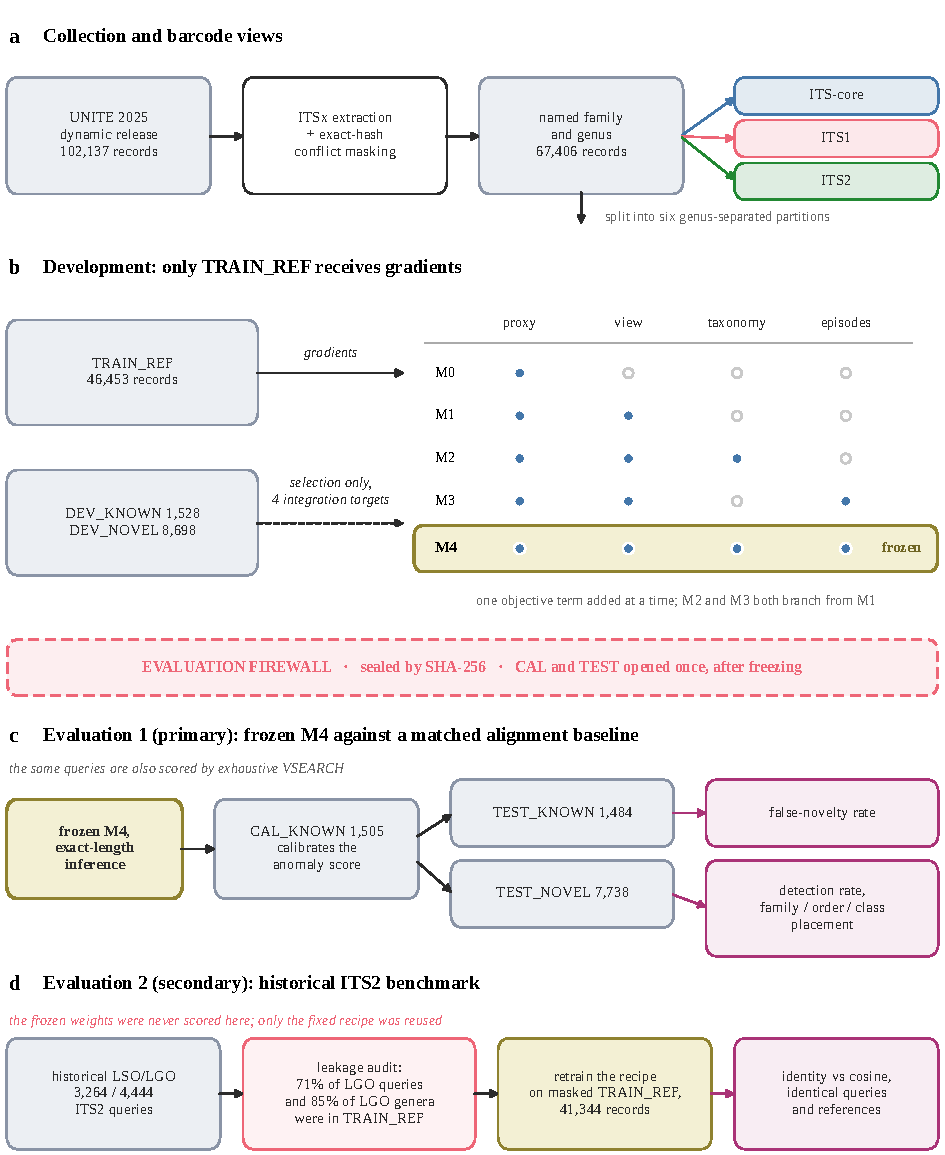
\includegraphics[width=\linewidth]{figures/fig1_workflow.pdf}
\caption{Design of the study. Fill colour marks the kind of object: grey for a
data partition, white for a process, yellow for a model, purple for a reported
result. (a) Collection, conflict masking and the three barcode views.
(b) Development: only TRAIN\_REF receives gradients, and the matrix gives the
objective terms of each rung (Appendix~\ref{app:ladder}). (c) The primary
evaluation, run once after freezing, in which the same queries are scored by the
frozen encoder with exact-length inference and by exhaustive VSEARCH identity.
(d) The historical benchmark: most of its held-out taxa had entered the original
training split, so the frozen weights were not scored there and the same recipe
was retrained on a masked TRAIN\_REF. The dashed band separates what was iterated
on from what was opened once.}
\label{fig:workflow}
\end{figure}

\subsection{Alignment baseline}
\label{sec:alignment}
Percent identity was computed with VSEARCH v2.31.0 \cite{rognes2016vsearch}.
VSEARCH ranks database sequences by the number of $k$-mers they share with the
query and aligns candidates in that order. Under the default
\texttt{--maxaccepts 1} it returns the first candidate that satisfies
\texttt{--id}; at \texttt{--id 0.5} that is usually the top $k$-mer candidate
rather than the highest-identity target, so \texttt{--top\_hits\_only} has no
effect and the reported value is not a best-hit identity. The default
\texttt{--maxrejects 32} also abandons a divergent query after 32 rejected
candidates. The sealed historical analysis used these defaults. Every other
identity score reported here used exhaustive search with a coverage
requirement:
\begin{quote}\small\ttfamily
vsearch --usearch\_global queries.fasta --db refs.fasta --id 0.5\\
--maxaccepts 0 --maxrejects 0 --top\_hits\_only --query\_cov 0.8\\
--threads 32 --userout hits.tsv --userfields query+target+id
\end{quote}
where 0 disables both termination heuristics. Among tied best hits the first
reported was kept. Depending on view, $1.5\%$ to $8.1\%$ of novel queries had
more than one tied best hit. Bracketing the tie rule, by counting a placement
correct only if every tied hit agreed with the query's lineage (the conservative,
lineage-aware reading) or if any did, changed novel-genus placement by at most
$0.2$ percentage points at any view and rank, so the choice of rule affects no
result. Queries with no
hit at identity $\geq0.5$ and query coverage $\geq0.8$ were retained, assigned a
score of $49.999\%$ for ranking, and counted as placement failures. VSEARCH
discarded five ITS1 and four ITS2 reference sequences shorter than its 32-nt
minimum. The coverage threshold was chosen after the unfiltered TEST placement
results had been seen, so we report the full threshold sweep rather than a
single value (Section~\ref{sec:baseline}).

The alignment baseline is paired with the encoder throughout: identical query
sets, identical reference collections, and the same split-conformal procedure,
with each score calibrated on its own CAL\_KNOWN values. For cross-view
retrieval, ITS1 or ITS2 queries were searched against the ITS-core references,
which contain both spacers, so an alignment can find the homologous region
directly.

\subsection{Paired uncertainty}
\label{sec:uncertainty}
AUROC differences were tested with the DeLong method \cite{delong1988} at the
query level. Because queries from one genus are strongly dependent, we also used
a paired genus-cluster bootstrap: known and novel genera were resampled
separately with replacement, every query in a sampled genus was carried at the
same weight, both scores received identical weights, and the weighted
Mann--Whitney AUROC was recomputed from scratch in each of $10{,}000$
replicates. Conformal decision rates were resampled in the same way, holding the
calibration scores fixed. Point estimates are query-weighted.

\subsection{Post-opening corrections and deviation log}
\label{sec:deviations}
Three corrections were made after the sealed evaluation had been opened: the
exact-length inference described above, the exhaustive VSEARCH configuration,
and the coverage filter. Each was recorded in a version-controlled deviation log
before any corrected metric was computed. The first entry was committed at 12:15
on 22 September 2026 (log SHA-256
\nolinkurl{f49548118ec4262a4dff430a68591b226efef0ee2daf4d72f153b9fa50ef6faf}),
and the first corrected TEST metrics were written at 12:33. A second entry,
pre-registering how a development rescore would be reported if M4 no longer met
its integration targets, was committed at 17:08 (SHA-256
\nolinkurl{ff80854b923f3963adfc07f3a791b0199b37cc285cf2d333aafb7e32ea844f73}),
one minute before the corrected development metrics were written. These
timestamps come from the authors' own machine and are not independently
attested. No model was
retrained, no threshold was tuned on TEST, and the sealed results are reported
beside the corrected ones throughout.

\subsection{Frozen conformal evaluation}
After M4 was frozen, CAL\_KNOWN alone calibrated the anomaly score. For a query
with anomaly $A(q)$ and calibration anomalies $A_1,\dots,A_{n_{\mathrm{cal}}}$,
the split-conformal $p$-value is
\begin{equation}
p(q)=\frac{1+\#\{i: A_i\ge A(q)\}}{n_{\mathrm{cal}}+1},
\label{eq:conformal}
\end{equation}
and queries with $p\le\alpha$ are called novel \cite{vovk2005,angelopoulos2023conformal}.
Under exchangeability of CAL\_KNOWN and a future known query, this conformal
$p$-value is super-uniform, so the marginal probability of a false novelty call
is at most $\alpha$. The empirical false-novelty fraction on a finite TEST\_KNOWN
sample may lie above or below $\alpha$. We report
$\alpha\in\{0.01,0.05,0.10,0.20\}$. TEST\_KNOWN supplies the observed
false-novelty rate and TEST\_NOVEL the detection rate, both per query and
averaged within novel genus. No DEV sequence was embedded or scored during the
locked evaluation.

\subsection{Historical benchmark and leakage audit}
The secondary benchmark uses the deposited leave-one-species-out (LSO) and
leave-one-genus-out (LGO) workflow of the companion novelty study
\cite{obrien2026flag}. On the historical $99{,}808$-sequence ITS2 FASTA, the
currently committed splitter generates $3{,}264$ LSO queries whose genus remains
represented and $4{,}444$ LGO queries whose family remains represented. The LGO
count reproduces the earlier analysis exactly. The earlier manuscript reported
$3{,}170$ LSO queries; the repository contains only one committed splitter
implementation, so the origin of that 94-query difference cannot be
reconstructed. We therefore treat the present $3{,}264/4{,}444$ split as a new
paired reproduction rather than a numerical reproduction of the earlier LSO run.

Before any neural scoring we audited whether the historical held-out taxa had
appeared in M4 training. They had, extensively: $3{,}166$ of $4{,}444$ exact LGO
queries, and 458 of the 538 held-out LGO genera, were present in the original
TRAIN\_REF (Table~\ref{tab:leakage}; Figure~\ref{fig:leakage}). We therefore did
not score the frozen M4 checkpoint on this benchmark. Instead, holding
architecture and hyperparameters fixed, we removed every historical LGO query
genus and every historical LSO query species from TRAIN\_REF and retrained the
same recipe without opening DEV, CAL or TEST. The mask removed $5{,}109$ records
($46{,}453\rightarrow41{,}344$); after view-availability filtering the training
runner used $41{,}065$ paired records covering $3{,}748$ genera, compared with
$46{,}150$ pairs and $4{,}231$ genera in the primary M4 run. The leakage-safe
model is therefore fitted to $11\%$ fewer records and $483$ fewer genera than
primary M4. Because DEV was not reopened for this run, how much that mask cost
in model quality is unmeasured. That is a deliberate price for keeping the
firewall closed rather than an oversight, but it qualifies the magnitude of the
comparison in Table~\ref{tab:historical} and is carried forward accordingly.

Identity on this benchmark used the same exhaustive, coverage-filtered search
as the primary evaluation (Section~\ref{sec:alignment}), and cosine used
exact-length inference on the leakage-safe checkpoint. The sealed analysis, run
with the default-settings search and padded inference, is deposited as
\texttt{data/historical\_benchmark\_sealed.csv}; correcting both arms moved the
AUROC difference from $+0.069$ to $+0.065$.
VSEARCH discarded five reference sequences shorter than its 32-nt minimum in
each benchmark search. Thirty LSO and 619 LGO queries had no hit at identity
$\geq0.5$ and query coverage $\geq0.8$ (21 and 542 under the default-settings
search); these queries were retained and assigned a score of 49.999\%
for ranking, representing censoring below the search threshold rather than an
estimated identity. M4 scored every query. The same half of the LSO queries
($n=1{,}632$), drawn by \texttt{np.random.default\_rng(0).permutation},
calibrated both scores; the other $1{,}632$ served as known test cases, and all
$4{,}444$ LGO queries served as the novel population. The halving determines
only which knowns calibrate and which are scored, but the operating points
depend on it: across ten halvings (seeds 0 to 9) the identity advantage ranged
from $+0.063$ to $+0.075$ AUROC, and every genus-clustered interval excluded
zero. Seed 0, reported throughout, lies near the low end of that range.

The known population in this benchmark is therefore the LSO query set, whose
species has been removed from the reference while its genus is retained. It is
species-novel rather than fully known, unlike TEST\_KNOWN in the primary
evaluation, which shifts the conformal null distribution and makes the absolute
operating points of the two evaluations non-comparable. The identity-versus-cosine
contrast within this benchmark is unaffected, because both scores are calibrated
and tested on exactly the same populations.

Because the deposited harness selects LSO and LGO queries under independent
protocols, the two populations are not disjoint. Of the $7{,}708$ query rows,
$336$ are sequences that appear in both arms; $182$ of these calibrate the
conformal threshold and also appear among the novel queries, and $281$ genera
are represented in both classes. Both scores are affected identically, so the
paired contrast is unaffected, but the conformal operating points on this
benchmark should be read as approximate.

% ============================================================================
% ============================================================================
\section{Results}
% ============================================================================
\subsection{The sealed evaluation reproduced exactly but was not batch-invariant}
\label{sec:invariance}
Rerunning the locked evaluator from the hash-verified checkpoint reproduced every
sealed value exactly. A second scoring script applied to the same checkpoint and
queries did not: maximum cosine similarities differed by a mean of $0.005$
(maximum $0.115$), and by more than $10^{-3}$ for $6{,}683$ of $10{,}679$
ITS-core queries, although the most discrepant input sequences were identical
(Table~\ref{tab:padding}). The cause was padding. Scoring TEST\_KNOWN ITS-core
queries one at a time, with no padding, moved maximum cosine by a mean of
$0.022$ relative to padded batches of 64, and padded values were lower by
$0.011$ on average; batches of 64 and 256, both heavily padded, differed by only
$0.004$. Between unpadded and padded scoring, $35.2\%$ of known queries changed
their nearest reference and $16.6\%$ changed its genus. Exact reproduction had
shown that the evaluation was consistent, not that it was invariant. Only a
second, independently batched scoring path could reveal the difference.

The artefact was largest where the sealed paper's cross-view claim lay.
Rescoring the M4 development matrix with exact-length inference lowered every
cross-view cell and left the same-view cells almost unchanged
(Table~\ref{tab:m4matrix}; data in \texttt{data/*\_sealed.csv}). Spacer-to-core
AUROC fell from $0.638$ and $0.660$ to $0.581$ and $0.616$, known-genus accuracy
from $44.9\%$ and $36.3\%$ to $32.9\%$ and $24.2\%$, and novel-family placement
from $39.2\%$ and $28.7\%$ to $30.0\%$ and $20.6\%$, whereas same-view AUROC
moved by at most $0.015$. This is consistent with padded normalisation adding a
component shared across views, so that embeddings of different barcode regions
looked more alike than they are. The artefact's effect on AUROC was also not
consistent in sign or size across partitions: correction lowered ITS2 AUROC by
$0.023$ on TEST, raised it by $0.003$ on DEV, and moved the historical ITS2
cosine AUROC by only $0.001$. It therefore cannot be corrected after the fact;
only batch-invariant inference removes it.

Correcting the inference moved the TEST AUROCs from \MsAUCCore{}, \MsAUCOne{}
and \MsAUCTwo{} to \MfAUCCore{}, \MfAUCOne{} and \MfAUCTwo{}
(Table~\ref{tab:headtohead}). The change was not symmetric noise: ITS-core rose
slightly, while both spacers fell by about $0.02$, so padding had been
flattering the spacer results specifically.

\begin{table}[htbp]\centering
\begin{threeparttable}
\caption{Dependence of M4 embeddings on inference batching, measured as the change in each query's maximum cosine to TRAIN\_REF. Same hash-verified checkpoint, same sequences, same device.}
\label{tab:padding}
\small
\begin{tabular}{lccc}
\toprule
comparison & mean $|\Delta|$ & max $|\Delta|$ & signed mean \\
\midrule
sealed evaluator vs second scoring script (all ITS-core) & 0.0054 & 0.115 & --- \\
batch 64 vs batch 256 (TEST\_KNOWN ITS-core) & 0.0045 & 0.080 & --- \\
batch 1 vs batch 64 (TEST\_KNOWN ITS-core) & 0.0220 & 0.146 & $-0.0110$ \\
batch 1 vs batch 256 (TEST\_KNOWN ITS-core) & 0.0226 & 0.151 & --- \\
sealed evaluator vs batch 1 (TEST\_KNOWN ITS-core) & 0.0226 & --- & $-0.0104$ \\
\bottomrule
\end{tabular}
\begin{tablenotes}\footnotesize
\item Batches of 64 and 256 are both heavily padded and differ little from each other; both differ from unpadded batch-1 inference by about five times as much. Between unpadded and padded scoring, 35.2\% of TEST\_KNOWN ITS-core queries changed their nearest reference and 16.6\% changed its genus. The magnitude of the shift correlates only weakly with sequence length (Spearman $\rho=-0.11$).
\end{tablenotes}
\end{threeparttable}
\end{table}


\subsection{The alignment baseline depends on its configuration}
\label{sec:baseline}
Two settings that are routinely left at their defaults each changed the
alignment baseline substantially (Table~\ref{tab:baseline};
Figure~\ref{fig:baselineconfig}). On the historical benchmark, the default
termination heuristics returned a different best hit from an exhaustive search
for \AudLgoPct{} of novel-genus queries and \AudLsoPct{} of known-genus ones,
with mean identity gains of \AudLgoGain{} and \AudLsoGain{} percentage points.
No hit ever worsened, as expected, since an exhaustive search cannot return a
worse best hit than a truncated one. Only five of the $542$ queries without a
default-settings hit gained one, so the censored set reflects genuinely
unalignable sequences rather than the rejection cap.

The second setting was the coverage requirement. Without it, ITS-core identity
placed novel genera in the correct family for only \CovNoneFam{} and the correct
class for \CovNoneCls{}, which inverted the ordering expected from barcode
length: ITS-core, which strictly contains both spacers, placed worse than
either. Requiring $80\%$ query coverage raised these to \CovEightFam{} and
\CovEightCls{} and restored the expected ordering, while changing ITS1 and ITS2
family placement by only $1.2$ and $3.8$ points and their order and class
placement not at all. The asymmetry identifies the cause. With no coverage
requirement, a distant reference that aligns well over the conserved 5.8S can
out-score a closer reference aligned across the full length; $44.5\%$ of
ITS-core best hits changed, with a mean identity change of $-2.53$ points, which
is the signature of higher-identity partial alignments being replaced by correct
full-length ones. The effect is insensitive to the exact threshold: order and
class plateau from $0.7$, and even $0.5$ recovers most of it.

Strikingly, the coverage filter left identity's novelty AUROC unchanged to three
decimals at every view (Table~\ref{tab:config}). An evaluation of the alignment
baseline by AUROC alone would therefore have reported a healthy baseline while
one ITS-core novel query in three was being assigned to the wrong class.

\begin{table}[htbp]\centering
\begin{threeparttable}
\caption{How the alignment baseline depends on its configuration. (a) Default termination heuristics against an exhaustive search on the historical ITS2 benchmark. (b) Query-coverage filtering on TEST\_NOVEL: the ITS-core rows sweep the threshold and the spacer rows are the control, since ITS1 and ITS2 contain no conserved region.}
\label{tab:baseline}
\footnotesize
\setlength{\tabcolsep}{4pt}
\begin{tabular}{lccccc}
\toprule
\multicolumn{6}{l}{\emph{(a) Default heuristics against exhaustive search, historical ITS2}} \\
query set & with a hit & lower-identity hit & target changed & rescued & mean gain \\
\midrule
LGO (novel genus) & 3,902 & 2,344 (60.1\%) & 2,419 (62.0\%) & 5 & $+2.93$ pp \\
LSO (known genus) & 3,243 & 1,108 (34.2\%) & 1,203 (37.1\%) & 0 & $+1.30$ pp \\
\midrule
\multicolumn{6}{l}{\emph{(b) Novel-genus placement by query-coverage filter, TEST}} \\
view & coverage filter & family & order & class & \\
\midrule
ITS-core & none & 53.7\% & 61.5\% & 64.9\% & \\
 & 0.5 & 73.1\% & 94.5\% & 96.3\% & \\
 & 0.7 & 81.2\% & 96.6\% & 98.4\% & \\
 & 0.8 & 84.6\% & 97.0\% & 98.6\% & \\
 & 0.9 & 85.8\% & 97.0\% & 98.7\% & \\
\addlinespace
ITS1 & none & 80.4\% & 94.4\% & 96.5\% & \\
 & 0.8 & 81.6\% & 94.4\% & 96.5\% & \\
\addlinespace
ITS2 & none & 76.2\% & 95.3\% & 97.6\% & \\
 & 0.8 & 80.0\% & 95.6\% & 97.5\% & \\
\bottomrule
\end{tabular}
\begin{tablenotes}\footnotesize
\item In (b), 44.5\% of ITS-core best hits changed between no filter and coverage $0.8$, with a mean identity change of $-2.53$ points: without the filter the search preferred higher-identity partial alignments that were taxonomically wrong. Identity AUROC was unchanged by the filter to three decimals at every view (Table~\ref{tab:config}). In (a), a lower-identity hit is one an exhaustive search improved on; a changed target also counts swaps among exact ties. Panel (b) is an independent search run: because multithreaded VSEARCH does not resolve exact ties deterministically, its $0.8$ row can differ from Table~\ref{tab:headtohead} by up to $0.1$ point.
\end{tablenotes}
\end{threeparttable}
\end{table}

\begin{table}[htbp]\centering
\begin{threeparttable}
\caption{The coverage filter changes placement and leaves novelty ranking untouched. Identity on TEST under exhaustive search, with and without query coverage $\geq0.8$.}
\label{tab:config}
\small
\begin{tabular}{llccc}
\toprule
view & configuration & AUROC & known genus NN & novel family \\
\midrule
ITS-core & exhaustive, no coverage filter & 0.7339 & 76.8\% & 53.7\% \\
 & exhaustive, query coverage 0.8 & 0.7338 & 83.4\% & 84.6\% \\
\addlinespace
ITS1 & exhaustive, no coverage filter & 0.7016 & 80.4\% & 80.4\% \\
 & exhaustive, query coverage 0.8 & 0.6997 & 80.9\% & 81.6\% \\
\addlinespace
ITS2 & exhaustive, no coverage filter & 0.7352 & 78.8\% & 76.2\% \\
 & exhaustive, query coverage 0.8 & 0.7349 & 80.8\% & 80.0\% \\
\bottomrule
\end{tabular}
\end{threeparttable}
\end{table}


\begin{figure}[htbp]\centering
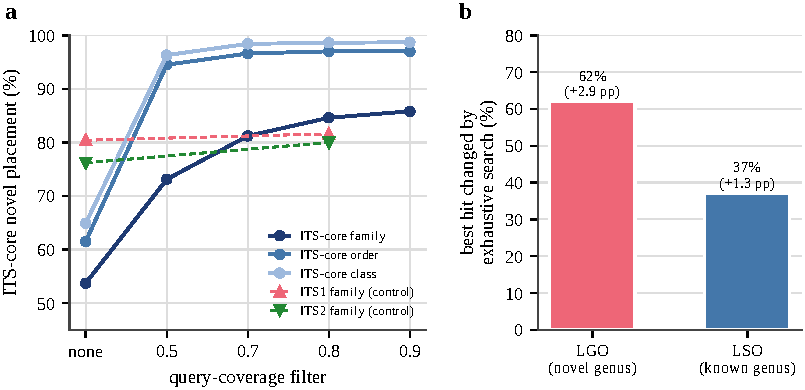
\includegraphics[width=\linewidth]{figures/fig7_baseline_config.pdf}
\caption{Configuration of the alignment baseline. (a) Best-hit placement of
ITS-core novel genera as the query-coverage filter is tightened; dashed lines
are the spacer controls, which contain no conserved region and barely move.
(b) Share of historical-benchmark queries whose best hit changed when the
default termination heuristics were replaced by an exhaustive search, with the
mean identity gain.}
\label{fig:baselineconfig}
\end{figure}

\subsection{A correctly configured alignment baseline matches or exceeds the
encoder on the primary split}
Scored on identical TEST queries and references, identity exceeded corrected M4
in known-genus nearest-neighbour accuracy at every view, \IdKnownCore{},
\IdKnownOne{} and \IdKnownTwo{} against \MfKnownCore{}, \MfKnownOne{} and
\MfKnownTwo{}, and in novel-family placement at every view, \IdFamCore{},
\IdFamOne{} and \IdFamTwo{} against \MfFamCore{}, \MfFamOne{} and \MfFamTwo{}
(Table~\ref{tab:headtohead}; Figure~\ref{fig:primary}). It also led at order and
class. The sealed M4 values, shown alongside, do not change this at any view.

Novelty ranking was close. M4's AUROC exceeded identity's by \DAUCCore{} at
ITS-core and \DAUCTwo{} at ITS2 and trailed by \DAUCOne{} at ITS1
(Table~\ref{tab:uncertainty}). At the query level only the ITS-core difference
was distinguishable from zero. The genus-cluster bootstrap widened every
interval roughly fivefold, to \GbLoCore{} to \GbHiCore{}, \GbLoOne{} to
\GbHiOne{}, and \GbLoTwo{} to \GbHiTwo{}, so no view shows a demonstrated
advantage for either score. The widening is itself informative: the novel
population contains thousands of queries but only \NGenCore{}, \NGenOne{} and
\NGenTwo{} genera, and the between-genus variation that the query-level analysis
ignores dominates the uncertainty. These intervals mean no demonstrated
advantage, not equivalence: they admit material differences in either
direction.

\begin{table}[htbp]\centering
\begin{threeparttable}
\caption{Primary TEST evaluation: M4 against a matched alignment baseline on identical queries and references. The sealed row is the locked evaluation as run, with padded inference; the corrected row recomputes the same checkpoint with exact-length batching. Identity is exhaustive VSEARCH with query coverage $\geq0.8$. Best value per view and column in bold.}
\label{tab:headtohead}
\small
\begin{tabular}{llccccc}
\toprule
 & & & known & \multicolumn{3}{c}{novel-genus placement} \\
\cmidrule(l){5-7}
view & score & AUROC & genus NN & family & order & class \\
\midrule
ITS-core & M4, sealed (padded) & 0.754 & 71.1\% & 65.0\% & 92.2\% & 97.3\% \\
 & M4, corrected & \textbf{0.756} & 71.2\% & 64.8\% & 92.5\% & 97.1\% \\
 & percent identity & 0.734 & \textbf{83.4\%} & \textbf{84.6\%} & \textbf{97.0\%} & \textbf{98.7\%} \\
\addlinespace
ITS1 & M4, sealed (padded) & \textbf{0.716} & 64.5\% & 55.2\% & 85.9\% & 94.0\% \\
 & M4, corrected & 0.699 & 61.6\% & 54.3\% & 84.4\% & 93.3\% \\
 & percent identity & 0.700 & \textbf{80.9\%} & \textbf{81.6\%} & \textbf{94.4\%} & \textbf{96.5\%} \\
\addlinespace
ITS2 & M4, sealed (padded) & \textbf{0.763} & 65.3\% & 52.0\% & 81.1\% & 92.9\% \\
 & M4, corrected & 0.740 & 66.2\% & 53.8\% & 81.7\% & 93.2\% \\
 & percent identity & 0.735 & \textbf{80.8\%} & \textbf{80.0\%} & \textbf{95.6\%} & \textbf{97.5\%} \\
\bottomrule
\end{tabular}
\begin{tablenotes}\footnotesize
\item $n$ known / novel: ITS-core 1,467/7,718; ITS1 1,477/7,702; ITS2 1,463/7,671. Identity censors queries with no hit at identity $\geq0.5$ and coverage $\geq0.8$ at $49.999$ and counts them as placement failures: ITS-core 0 known, 0 novel; ITS1 26 known, 118 novel; ITS2 7 known, 78 novel.
\item Paired uncertainty for the AUROC and detection contrasts is in Table~\ref{tab:uncertainty}.
\end{tablenotes}
\end{threeparttable}
\end{table}

\begin{table}[htbp]\centering
\begin{threeparttable}
\caption{Paired uncertainty for corrected M4 against identity on TEST, M4 minus identity. The query-level DeLong interval treats queries as independent; the genus-cluster bootstrap resamples whole genera separately within the known and novel classes, applies identical weights to both scores, and uses 10,000 replicates.}
\label{tab:uncertainty}
\footnotesize
\setlength{\tabcolsep}{4pt}
\begin{tabular}{lccccc}
\toprule
\multicolumn{6}{l}{\emph{(a) Novelty AUROC}} \\
view & $\Delta$AUROC & DeLong 95\% CI & $P$ & genus 95\% CI & Bonferroni, 3 views \\
\midrule
ITS-core & $+0.022$ & $+0.012$ to $+0.033$ & $4.1\times10^{-5}$ & $-0.069$ to $+0.104$ & $-0.073$ to $+0.115$ \\
ITS1 & $-0.001$ & $-0.014$ to $+0.012$ & $0.878$ & $-0.116$ to $+0.097$ & $-0.124$ to $+0.112$ \\
ITS2 & $+0.005$ & $-0.005$ to $+0.015$ & $0.357$ & $-0.069$ to $+0.068$ & $-0.074$ to $+0.076$ \\
\midrule
\multicolumn{6}{l}{\emph{(b) Novel detection at nominal $\alpha=0.05$}} \\
view & M4 & identity & $\Delta$, pp & genus 95\% CI & false novelty, M4 / identity \\
\midrule
ITS-core & 6.0\% & 14.6\% & $-8.7$ & $-19.7$ to $+0.2$ & 3.7\% / 3.2\% \\
ITS1 & 5.5\% & 8.4\% & $-2.9$ & $-9.5$ to $-0.1$ & 4.9\% / 4.0\% \\
ITS2 & 9.6\% & 14.9\% & $-5.3$ & $-13.5$ to $+1.3$ & 4.3\% / 3.4\% \\
\bottomrule
\end{tabular}
\begin{tablenotes}\footnotesize
\item Novel genera per view: ITS-core 183, ITS1 184, ITS2 183. Point estimates are query-weighted; the genus-cluster interval is for a genus-resampled version of that statistic. Rate intervals hold the CAL\_KNOWN scores fixed, so they omit calibration-set sampling variability and understate total uncertainty.
\item An interval that includes zero means no demonstrated advantage, not equivalence.
\end{tablenotes}
\end{threeparttable}
\end{table}


\begin{figure}[htbp]\centering
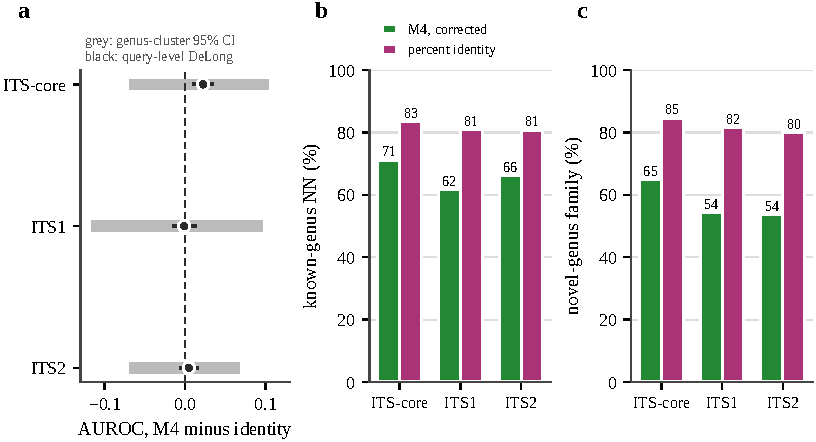
\includegraphics[width=\linewidth]{figures/fig4_primary.pdf}
\caption{Corrected M4 against percent identity on identical TEST queries.
(a) AUROC difference, M4 minus identity, with the query-level DeLong interval
(black) and the genus-cluster bootstrap interval (grey). (b) Known-genus
nearest-neighbour accuracy. (c) Novel-genus family placement.}
\label{fig:primary}
\end{figure}

\subsection{Identity dominates at every deployable operating point}
At $\alpha=0.05$, identity detected \IdDetCore{}, \IdDetOne{} and \IdDetTwo{} of
novel-genus queries against M4's \MfDetCore{}, \MfDetOne{} and \MfDetTwo{}, at
observed false-novelty rates of \IdFnCore{}, \IdFnOne{} and \IdFnTwo{} against
\MfFnCore{}, \MfFnOne{} and \MfFnTwo{} (Table~\ref{tab:operating};
Figure~\ref{fig:operating}). Identity therefore detected more and erred less
simultaneously, at every view, and the pattern held at $\alpha=0.10$. At
$\alpha=0.01$ both scores detected almost nothing, and ITS1 identity flagged no
query at all. Under genus-cluster resampling the detection difference at
$\alpha=0.05$ excluded zero at ITS1 and narrowly included it at ITS-core and
ITS2.

This is the sharpest form of a point that applies well beyond this study.
M4's AUROC was comparable to identity's, yet M4 was dominated in both
coordinates at every operating point in the usable range. AUROC integrates over
the whole curve, including high-error regions no user would choose; the
decision a user makes is taken at a single stringent threshold. Novelty scores
for barcoding should be compared at the operating points at which they would be
deployed.

The novel genera flagged by the two methods at $\alpha=0.05$ overlapped only
partly, with Jaccard indices of $0.17$ to $0.23$ and Spearman correlations
between the scores of $0.61$ to $0.72$, so the two scores are not redundant.
Their naive union was nonetheless worse than identity alone: flagging a query
when either score did so detected $17.0\%$, $11.9\%$ and $20.0\%$ of novel
queries at observed false-novelty rates of $5.9\%$, $7.9\%$ and $6.6\%$, whereas
identity alone, interpolated to the same error rates, detected about $25\%$,
$26\%$ and $27\%$. Any useful combination would require a rule fixed in advance
and validated on a fresh holdout.

\begin{table}[htbp]\centering
\begin{threeparttable}
\caption{Conformal operating points on TEST for corrected M4 and identity, each calibrated on its own CAL\_KNOWN scores by the same procedure. False novelty is the fraction of TEST\_KNOWN flagged; detection the fraction of TEST\_NOVEL flagged.}
\label{tab:operating}
\small
\begin{tabular}{llcccc}
\toprule
 & & \multicolumn{2}{c}{M4, corrected} & \multicolumn{2}{c}{percent identity} \\
\cmidrule(lr){3-4}\cmidrule(lr){5-6}
view & $\alpha$ & false novelty & detection & false novelty & detection \\
\midrule
ITS-core & 0.01 & 0.2\% & \textbf{0.7\%} & 0.5\% & 0.3\% \\
 & 0.05 & 3.7\% & 6.0\% & 3.2\% & \textbf{14.6\%} \\
 & 0.10 & 8.4\% & 18.4\% & 7.2\% & \textbf{30.9\%} \\
 & 0.20 & 17.6\% & \textbf{45.3\%} & 16.4\% & 45.2\% \\
\addlinespace
ITS1 & 0.01 & 0.4\% & \textbf{0.8\%} & 0.0\% & 0.0\% \\
 & 0.05 & 4.9\% & 5.5\% & 4.0\% & \textbf{8.4\%} \\
 & 0.10 & 8.7\% & 12.3\% & 7.4\% & \textbf{24.8\%} \\
 & 0.20 & 18.1\% & 30.6\% & 16.9\% & \textbf{45.4\%} \\
\addlinespace
ITS2 & 0.01 & 0.8\% & \textbf{1.2\%} & 0.5\% & 1.1\% \\
 & 0.05 & 4.3\% & 9.6\% & 3.3\% & \textbf{15.0\%} \\
 & 0.10 & 8.6\% & 21.4\% & 7.6\% & \textbf{31.0\%} \\
 & 0.20 & 17.5\% & 41.1\% & 17.2\% & \textbf{44.9\%} \\
\bottomrule
\end{tabular}
\begin{tablenotes}\footnotesize
\item Higher detection per row in bold. At $\alpha\in\{0.05,0.10\}$ identity detects more novel queries at a lower observed false-novelty rate at every view. At $\alpha=0.01$ both scores detect almost nothing, and ITS1 identity flags no query at all.
\end{tablenotes}
\end{threeparttable}
\end{table}


\begin{figure}[htbp]\centering
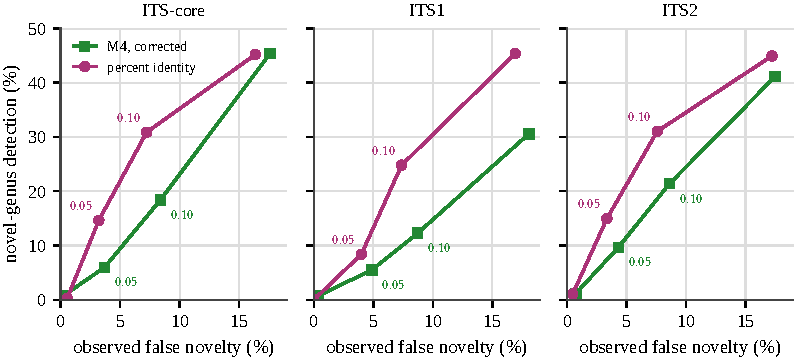
\includegraphics[width=\linewidth]{figures/fig5_operating.pdf}
\caption{Conformal operating points on TEST. Each curve joins the nominal
levels $\alpha=0.01$, $0.05$, $0.10$ and $0.20$; the $0.05$ and $0.10$ points
are labelled. A curve above and to the left of another dominates it. Identity
dominates corrected M4 throughout the usable range at all three views.}
\label{fig:operating}
\end{figure}

\subsection{Cross-view retrieval is available to alignment through ITS-core}
The sealed evaluation's strongest cross-view results were retrieval of ITS1 or
ITS2 queries against ITS-core references (Table~\ref{tab:m4matrix}). Because
ITS-core contains both spacers, that comparison is homologous by construction,
and an alignment can make it directly. On the same development queries and
references, exhaustive identity reached known-genus accuracy of
\XIdKnownOne{} and \XIdKnownTwo{} against M4's \XMKnownOne{} and \XMKnownTwo{},
novel-family placement of \XIdFamOne{} and \XIdFamTwo{} against \XMFamOne{} and
\XMFamTwo{}, and AUROC of \XIdAUCOne{} and \XIdAUCTwo{} against \XMAUCOne{} and
\XMAUCTwo{} (Table~\ref{tab:crossview}). M4 was selected on these partitions, so
these cells if anything flatter it, and the gaps are 47 to 54 points in genus
accuracy and 41 to 49 in family placement. The one cross-view comparison
alignment cannot make, direct ITS1-to-ITS2 retrieval, is also the one at which
M4 performs at chance, with AUROCs of $0.490$ and $0.471$. The model's cross-view ability is
therefore core-anchored, and in the direction that matters it reproduces, less
well, a retrieval alignment performs without training.

\begin{table}[htbp]\centering
\begin{threeparttable}
\caption{Cross-view retrieval through the ITS-core references on DEV. Spacer queries searched against ITS-core references, by exhaustive VSEARCH (query coverage $\geq0.8$) and by M4 cosine. Because ITS-core contains both spacers, this is a homologous comparison that alignment can make directly.}
\label{tab:crossview}
\small
\begin{tabular}{llccc}
\toprule
query view & score & AUROC & known genus NN & novel family \\
\midrule
ITS1 & percent identity & \textbf{0.801} & \textbf{79.8\%} & \textbf{70.9\%} \\
 & M4 cosine & 0.581 & 32.9\% & 30.0\% \\
\addlinespace
ITS2 & percent identity & \textbf{0.779} & \textbf{78.5\%} & \textbf{69.8\%} \\
 & M4 cosine & 0.616 & 24.2\% & 20.6\% \\
\bottomrule
\end{tabular}
\begin{tablenotes}\footnotesize
\item M4 values use exact-length inference; under the sealed, padded inference they were about 12 points higher in genus accuracy and 8 to 9 in family placement (Section~\ref{sec:invariance}). M4 was selected on DEV, so these cells if anything flatter it. Direct ITS1-to-ITS2 retrieval, the only genuinely non-homologous pair, has M4 AUROC $0.490$ and $0.471$ (Table~\ref{tab:m4matrix}).
\end{tablenotes}
\end{threeparttable}
\end{table}


\subsection{The development-to-TEST gap is partition composition, not selection}
M4's development AUROCs lie above its corrected TEST values at every view, by
\MfGapCore{}, \MfGapOne{} and \MfGapTwo{} (Table~\ref{tab:devtest}). A learned
score cannot separate selection optimism from a difference between partitions
on its own, so we scored identity on both. Identity is parameter-free and
nothing was selected on it, so its development-to-TEST gap estimates partition
composition alone. That gap was larger than M4's at every view, \IdGapCore{},
\IdGapOne{} and \IdGapTwo{}, leaving no positive residual to attribute to
selection. Family placement agreed: both scores were 7 to 14 points lower on
DEV\_NOVEL than on TEST\_NOVEL. DEV\_NOVEL is simply the easier partition for
novelty ranking and the harder one for placement. Every value in this
comparison uses exact-length inference or exhaustive search. A development-above-test
gap is often read as selection optimism; here a parameter-free control shows
that reading to be wrong on the data that produced it.

\begin{table}[htbp]\centering
\begin{threeparttable}
\caption{Development-to-TEST movement separated into partition composition and selection. Identity is parameter-free and nothing was selected on it, so its gap estimates composition alone. Same-view retrieval throughout.}
\label{tab:devtest}
\small
\begin{tabular}{lcccccccc}
\toprule
 & \multicolumn{3}{c}{identity AUROC} & \multicolumn{3}{c}{M4 AUROC} & residual & \\
\cmidrule(lr){2-4}\cmidrule(lr){5-7}
view & DEV & TEST & gap & DEV & TEST & gap & (M4 $-$ identity) & \\
\midrule
ITS-core & 0.809 & 0.734 & $+0.075$ & 0.777 & 0.756 & $+0.021$ & $-0.054$ & \\
ITS1 & 0.806 & 0.700 & $+0.107$ & 0.740 & 0.699 & $+0.041$ & $-0.066$ & \\
ITS2 & 0.778 & 0.735 & $+0.044$ & 0.754 & 0.740 & $+0.014$ & $-0.029$ & \\
\addlinespace
\multicolumn{9}{l}{\emph{Novel-family placement, DEV minus TEST}} \\
ITS-core & \multicolumn{8}{l}{identity $-8.8$ pp; M4 $-7.2$ pp} \\
ITS1 & \multicolumn{8}{l}{identity $-10.8$ pp; M4 $-9.2$ pp} \\
ITS2 & \multicolumn{8}{l}{identity $-10.7$ pp; M4 $-13.4$ pp} \\
\bottomrule
\end{tabular}
\begin{tablenotes}\footnotesize
\item Both scores use corrected inference throughout: exact-length batching for M4 and exhaustive, coverage-filtered search for identity. No view shows a positive residual.
\end{tablenotes}
\end{threeparttable}
\end{table}


\subsection{A historical benchmark was contaminated by training data}
The secondary benchmark reuses the leave-one-genus-out and
leave-one-species-out workflow of our companion study, built from the same
UNITE release. Before scoring it we audited whether its held-out taxa had
appeared in M4 training. $3{,}166$ of the $4{,}444$ novel-genus queries ($71\%$)
and 458 of the 538 held-out genera ($85\%$) were present in the original
TRAIN\_REF (Table~\ref{tab:leakage}; Figure~\ref{fig:leakage}). Scoring the
frozen checkpoint on this benchmark would have measured recall of training data
under the name of novelty detection. We therefore retrained the fixed recipe on
a TRAIN\_REF with every leaked taxon removed. The mechanism is general: any
leave-one-taxon-out benchmark derived from the same release as a model's
training data will leak unless exclusions are enforced before training rather
than at evaluation. On the leakage-safe benchmark, identity again outperformed the retrained model,
and here the difference is statistically clear. AUROC was $0.768$ against
$0.703$, a difference of $+0.065$ whose genus-clustered interval, resampling 538
novel and 1,387 known genera, ran from $+0.046$ to $+0.085$
(Table~\ref{tab:historical}; Figure~\ref{fig:historical}). At $\alpha=0.05$
identity detected $28.2\%$ of novel-genus queries against $11.2\%$, with 872
queries flagged by identity alone and 117 by cosine alone, and it recovered the
correct family for $52.6\%$ of them against $28.2\%$. About half of identity's
detections were queries with no alignable reference at all. Two features of the
benchmark plausibly make it harsher for the model than the primary split: the
retrained checkpoint was fitted to $11\%$ fewer records and 483 fewer genera,
and its known class consists of held-out species rather than known genera.
% ============================================================================
\section{Discussion}
% ============================================================================
Every comparison between the learned embedding and a correctly configured
alignment baseline either favoured alignment or showed no demonstrated
difference. Alignment placed novel genera more accurately at every view and
rank, identified known genera more accurately, detected more novel genera at a
lower error rate at every usable threshold, and performed the cross-view
retrievals credited to the embedding far better. The embedding retained a novelty
AUROC close to identity's, which the operating-point analysis showed to be the
least decision-relevant of the metrics examined.

The reason is not mysterious. For homologous queries and references, alignment
compares sequences at full nucleotide resolution. The encoder compresses the
same information into 256 dimensions while being asked to satisfy locus
invariance, genus discrimination and hierarchical structure at once. Where the
compression could in principle add something alignment lacks, in a shared space
for non-homologous barcode views, the model performed near chance, because the
cross-view structure it did learn was anchored on the ITS-core region that
alignment can use directly.

The more transferable result concerns the evaluation. The sealed evaluation was
carefully designed, with a genus-separated split, a sealed test set, a hash
check and preregistered integration targets, and it still supported a
conclusion that did not survive. Each correction that changed it is inexpensive:
\begin{enumerate}\itemsep0pt
\item Score a non-learned baseline on the same split, not only weaker versions
of the model.
\item Configure that baseline as a user would for best-hit assignment:
exhaustive search, and a coverage requirement when the barcode contains a
conserved region. Report the configuration.
\item Compare novelty scores at deployable operating points, not only by AUROC,
which here was blind both to a broken baseline and to a dominated model.
\item Compute uncertainty at the level of the unit that is actually independent,
here the genus.
\item Test whether embeddings are invariant to inference batching by scoring the
same queries through two independently batched paths.
\item Use a parameter-free score as the control for selection optimism.
\item Audit any benchmark for training-set leakage before scoring it.
\end{enumerate}
None of these requires a new method. Each changed a conclusion here, and several
would have been invisible without the others: the coverage artefact was
invisible to AUROC, and the padding effect was invisible to exact
reproduction.

\subsection{Relation to prior work}
Orsholm et al.\ compared classifiers for unknown barcodes across animal COI and
fungal ITS and found composition-based classifiers strongest for fungal ITS,
with alignment-threshold methods over-assigning queries to novel branches
\cite{orsholm2026unseen}. Our results are consistent with theirs on the
importance of baseline configuration and complementary in scope: they compared
classification rules across many methods, whereas we examined how evaluation
choices decide a single learned-versus-alignment comparison. Zero-shot and
hierarchical Bayesian models for insect barcodes
\cite{badirli2021zeroshot,badirli2023classifying} and out-of-distribution
detection for insect barcoding \cite{fujisawa2026ood} share our motivation, and
the last reaches a compatible conclusion, that learned scores do not
automatically dominate distance baselines. Benchmark design has shaped earlier conclusions in the same way. Edgar's
cross-validation-by-identity benchmark for 16S and fungal ITS found that
newer classification algorithms did not improve on the RDP classifier or
SINTAX \cite{edgar2018accuracy}, and the SINTAX evaluation showed most methods
assigning known names to novel taxa \cite{edgar2016sintax}. Our results extend
that line from classification rules to learned representations. Established
probabilistic classifiers with explicit novelty handling, including PROTAX-Fungi
\cite{abarenkov2018protax} and BayesANT \cite{zito2023bayesant}, and
composition classifiers such as SINTAX \cite{edgar2016sintax}, are the natural
next baselines for the protocol described here.

\subsection{Limitations}
\label{sec:limitations}
All experiments use one UNITE release. The strongest test of generalisation,
training on an earlier release and evaluating taxa that first appear in a later
one, remains to be done, and would also address whether learned barcode
embeddings largely memorise their training set.

The leakage-safe retrain was not re-evaluated on DEV, so the cost of the
exclusion mask to model quality is unmeasured, and the historical comparison may
understate what an unmasked model would achieve on genuinely novel taxa.

The ladder was run at a single seed, so small differences between adjacent rungs
are not separable from run-to-run variation. The genus-cluster bootstrap assumes
genera are independent within each class and ignores family-level dependence,
and its rate intervals hold the calibration set fixed, so they understate total
uncertainty. The coverage threshold was chosen after unfiltered TEST placement
had been seen; the sweep shows the conclusion does not depend on the value, and
the filter improves the baseline rather than the model under study. We reported
all three barcode views with equal weight and did not select among them after
seeing results.

\section{Conclusions}
A purpose-trained fungal ITS embedding did not outperform correctly configured
alignment on any comparison we could make, and fell well short of it on
higher-rank placement, genus identification, deployable novelty detection and
cross-view retrieval. The comparison was decided by evaluation choices: how the
alignment baseline was configured, whether the embedding was invariant to
batching, whether uncertainty was computed at the genus level, whether a
parameter-free control was used for selection, and whether the benchmark had
leaked into training. These checks are general and inexpensive, and we suggest
that learned barcode methods be reported against them.

\section*{Data and code availability}
Code, the deviation log with its commit history, and the environment files are
deposited in a public repository\todo{repository URL and archival DOI}. Every table, figure and
quoted number in this manuscript is regenerated from the CSV files in
\texttt{manuscript/data} by \texttt{manuscript/analysis/make\_tables.py},
\texttt{make\_figures.py} and \texttt{make\_primary.py}; the historical-benchmark
CSV is itself rebuilt from the per-query score table and the raw best-hit
tables by \texttt{analysis/rebuild\_historical\_benchmark.py}, and the per-query
table by \texttt{scripts/build\_historical\_per\_query.py}. Model checkpoints,
the split table, and the per-query predictions and search hits are deposited
separately\todo{data deposit DOI}. The sequence source is the UNITE general
FASTA release for Fungi of 19 February 2025 \cite{unite2025release}.

\section*{Funding}
This work was carried out at the Centro de Biotecnolog\'ia de Sistemas,
Universidad Andr\'es Bello, under CORFO grant 23PTECCC-247149.

\section*{Author contributions}
Aaron O'Brien: conceptualization, methodology, software, formal analysis,
investigation, data curation, visualization, writing (original draft), writing
(review and editing). Auguste Gardette: conceptualization, methodology,
validation, writing (review and editing). A.G.\ contributed to the conception of
the study and proposed its framing as an evaluation protocol. His review
identified the absence of a non-learned baseline on the primary split, the
homologous confounder in cross-view retrieval, and the termination behaviour of
the default VSEARCH search, each of which led to an analysis reported here. Both
authors read and approved the submitted version. \verify{A.G.\ to confirm.}

\section*{Acknowledgements}
We thank the UNITE community for curating and releasing the reference data on
which every experiment here depends.

\section*{Competing interests}
The authors declare no competing interests.

\section*{Use of generative AI}
Anthropic's Claude and GitHub Copilot were used in preparing this work: to
draft and revise manuscript text, to write and debug the analysis and figure
scripts deposited with it, and to check bibliographic details. All analyses
were run by the authors, all reported values were verified against the primary
output, and the authors are responsible for the content of the manuscript.

% ============================================================================
\appendix
\renewcommand{\thetable}{S\arabic{table}}
\renewcommand{\thefigure}{S\arabic{figure}}
\renewcommand{\theHtable}{S\arabic{table}}
\renewcommand{\theHfigure}{S\arabic{figure}}
\setcounter{table}{0}
\setcounter{figure}{0}

\section{Reproducibility, frozen artefacts and supplementary results}
\label{app:repro}
The primary frozen M4 checkpoint SHA-256 is\\
\nolinkurl{e4cf8bfed197b2b15758a93798c025a2a482e5ad81c5965b376bcf4bb237671f}.\\
The split TSV SHA-256 is\\
\nolinkurl{27041e67b8db254c31a8fcb4001b35c07486786777d6ce09a21a86c4997cb411}.\\
The locked final evaluator embedded TRAIN\_REF, CAL\_KNOWN, TEST\_KNOWN and
TEST\_NOVEL but did not embed or score DEV. The historical-safe retraining used
the selected M4 recipe unchanged and skipped DEV, CAL and TEST evaluation
entirely. The leakage-safe checkpoint scored in Table~\ref{tab:historical} has
SHA-256\\
\nolinkurl{99b91448b0401acbc6d007156df08dc85420036bffdc80ef54746c11280de16a}.\\
Each corrected evaluation records its evaluator and model-source hashes and its
inference policy in its output metadata, and every one of those hashes matches
the corresponding file deposited in the repository.

Neural training was run with PyTorch 2.14.0+cu130 on an NVIDIA GeForce RTX 5070
Ti with CUDA 13.0; ITS extraction used ITSx 1.1.3. The training environment is
deposited as \texttt{environment.lock}. The corrected evaluation and all
analyses ran on Python 3.13.12 (conda-forge), PyTorch 2.14.0 with CUDA 13.0,
NumPy 2.5.3, pandas 3.0.6 and SciPy 1.18.1, on the same GPU (driver 595.84), with
VSEARCH v2.31.0; the full package list is deposited as
\texttt{environment/requirements.txt}. Hashes prove that an artefact did not
change; the environment files are what make it rebuildable.

The run logs deposited with the code date each fit of the ladder: M0 through M3
completed between 12:34 and 13:48 on 11 September 2026 and M4 began at 13:57, so
the sequence on which the integration targets depend is checkable from the
artefacts rather than only asserted. The threshold values themselves were fixed
in working notes in that interval and are not independently timestamped
($\S$\ref{sec:split}).
Paired uncertainty for the historical benchmark is computed by
\texttt{analysis/paired\_uncertainty.py}, which reports a clustered paired
bootstrap interval for the AUROC difference, the DeLong test for the same
contrast, and McNemar's test on the conformal flag sets at each $\alpha$.

\begin{table}[htbp]\centering
\begin{threeparttable}
\caption{Sensitivity of the hierarchical objective to its weight. The reduced $\lambda_{\mathrm{tax}}=0.25$ run was performed once after the initially specified $\lambda_{\mathrm{tax}}=1.0$ run and was not followed by a weight sweep.}
\label{tab:m2sens}
\begin{tabular}{llccc}
\toprule
$\lambda_{\mathrm{tax}}$ & view & AUROC & novel family & novel order \\
\midrule
1.00 & ITS-core & 0.752 & 35.8\% & 60.8\% \\
 & ITS1 & 0.740 & 32.7\% & 56.9\% \\
 & ITS2 & 0.740 & 31.5\% & 56.9\% \\
\addlinespace
0.25 & ITS-core & 0.748 & 33.6\% & 58.7\% \\
 & ITS1 & 0.736 & 28.8\% & 52.2\% \\
 & ITS2 & 0.723 & 29.7\% & 53.8\% \\
\bottomrule
\end{tabular}
\begin{tablenotes}\footnotesize
\item Reducing the weight to one quarter lowered AUROC and every placement metric at every view. The sensitivity run therefore did not motivate further DEV-set weight tuning.
\end{tablenotes}
\end{threeparttable}
\end{table}

\begin{table}[htbp]\centering
\begin{threeparttable}
\caption{Historical-benchmark leakage audit and exclusion mask. The share column expresses each count as a percentage of the corresponding held-out set.}
\label{tab:leakage}
\begin{tabular}{lrr}
\toprule
item & count & share of held-out set \\
\midrule
\multicolumn{3}{l}{\emph{Training records}} \\
\quad original TRAIN\_REF & 46,453 & \\
\quad leakage-safe TRAIN\_REF & 41,344 & \\
\quad excluded by the mask & 5,109 & \\
\addlinespace
\multicolumn{3}{l}{\emph{Leave-one-genus-out (LGO) queries}} \\
\quad queries & 4,444 & \\
\quad query genera & 538 & \\
\quad exact query IDs in original TRAIN\_REF & 3,166 & 71.2\% \\
\quad query genera in original TRAIN\_REF & 458 & 85.1\% \\
\quad query genera after the mask & 0 & 0.0\% \\
\quad exact query IDs after the mask & 0 & 0.0\% \\
\addlinespace
\multicolumn{3}{l}{\emph{Leave-one-species-out (LSO) queries}} \\
\quad queries & 3,264 & \\
\quad query species & 2,541 & \\
\quad exact query IDs in original TRAIN\_REF & 2,107 & 64.6\% \\
\quad query species in original TRAIN\_REF & 1,694 & 66.7\% \\
\quad query species after the mask & 0 & 0.0\% \\
\quad query genera still represented after the mask & 1,887 & \\
\bottomrule
\end{tabular}
\begin{tablenotes}\footnotesize
\item The LSO design deliberately keeps the query's genus in the reference collection, so the last row is a property of the design rather than residual leakage. What the mask had to remove was the query species itself.
\end{tablenotes}
\end{threeparttable}
\end{table}


\begin{figure}[htbp]\centering
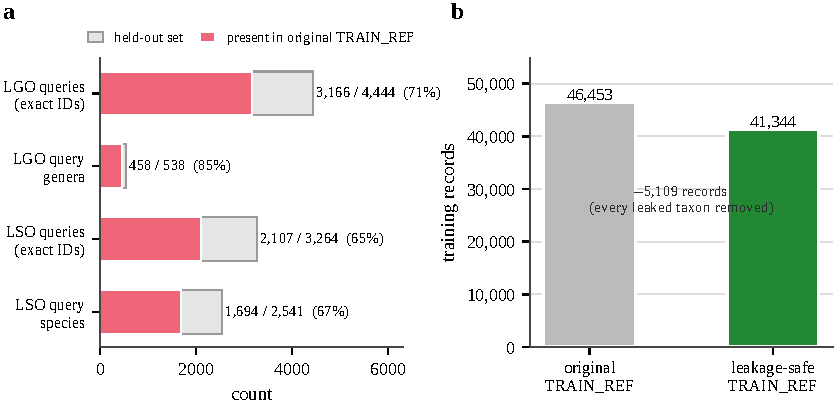
\includegraphics[width=\linewidth]{figures/figS1_leakage_audit.pdf}
\caption{Why the frozen checkpoint could not be scored on the historical
benchmark. (a) Most nominally held-out historical queries and query taxa were
already present in the original TRAIN\_REF. (b) Removing every one of them cost
$5{,}109$ training records and brought residual leakage to zero, after which the
fixed M4 recipe was retrained.}
\label{fig:leakage}
\end{figure}


\section{Development ladder and training objectives}
\label{app:ladder}
\subsection{Training objectives}
Let a training batch contain $B$ source records. Each record contributes an
ITS-core embedding $z_i^{c}$ and one randomly selected available spacer
embedding $z_i^{a}$ (ITS1 or ITS2). Let $w_g$ denote a learned, L2-normalized
proxy for genus $g$.

\noindent\emph{Genus proxy (all models).} The genus head is a
cosine-softmax classifier evaluated on ITS-core only:
\begin{equation}
\mathcal{L}_{\mathrm{proxy}}
= -\frac{1}{B}\sum_{i=1}^{B}
\log\frac{\exp\!\left(\cos(z_i^c,w_{g_i})/\tau_g\right)}
{\sum_{g\in G}\exp\!\left(\cos(z_i^c,w_g)/\tau_g\right)},
\label{eq:proxy}
\end{equation}
with $\tau_g=0.07$.

\noindent\emph{Cross-view invariance (M1--M4).} The implementation uses a
symmetric supervised-contrastive objective over all $2B$ views in the batch. If
$\pi(a)$ denotes the other view from the same source record as anchor $a$, then
\begin{equation}
\mathcal{L}_{\mathrm{view}}
= -\frac{1}{2B}\sum_{a=1}^{2B}
\log\frac{\exp\!\left(\cos(z_a,z_{\pi(a)})/\tau_v\right)}
{\sum_{b\neq a}\exp\!\left(\cos(z_a,z_b)/\tau_v\right)}.
\label{eq:view}
\end{equation}
Thus both core$\rightarrow$spacer and spacer$\rightarrow$core directions are
anchors, and every non-self view in the minibatch enters the denominator. We
used $\tau_v=0.10$.

\noindent\emph{Hierarchical taxonomic geometry (M2, M4).} This term acts on
pairwise ITS-core embeddings within the minibatch, not on genus proxies. For
records $i$ and $j$, let $h_{ij}\in\{0,\ldots,6\}$ be the number of consecutive
ranks shared when their lineages are traversed from phylum toward species until
the first mismatch, and define $d_{ij}=6-h_{ij}$. For $j\neq i$, the target and
embedding-neighbour distributions are
\begin{equation}
p_{ij}=\frac{\exp(-\beta d_{ij})}{\sum_{k\neq i}\exp(-\beta d_{ik})},
\qquad
q_{ij}=\frac{\exp(\cos(z_i^c,z_j^c)/\tau_t)}
{\sum_{k\neq i}\exp(\cos(z_i^c,z_k^c)/\tau_t)},
\end{equation}
and
\begin{equation}
\mathcal{L}_{\mathrm{tax}}
= -\frac{1}{B}\sum_i\sum_{j\neq i} p_{ij}\log q_{ij}.
\label{eq:tax}
\end{equation}
We used $\tau_t=0.10$ and $\beta=0.70$.

\noindent\emph{Leave-one-genus family episodes (M3, M4).} Family prototypes
are constructed from all learned genus proxies. Writing
$s_F=\sum_{g\in F}w_g$ and $c_F=\mathrm{norm}(s_F)$, an eligible query from
genus $g_i$ and family $F_i$ replaces only its true-family prototype with
\begin{equation}
c_{F_i}^{-g_i}=\mathrm{norm}(s_{F_i}-w_{g_i}),
\end{equation}
which explicitly removes the query genus. Families represented by only one genus
are skipped. The query is classified over all represented families, using
$c_{F_i}^{-g_i}$ for the target logit and ordinary $c_F$ for every non-target
family:
\begin{equation}
\mathcal{L}_{\mathrm{epi}}
= -\frac{1}{|E|}\sum_{i\in E}
\log\frac{\exp(\cos(z_i^c,c_{F_i}^{-g_i})/\tau_e)}
{\exp(\cos(z_i^c,c_{F_i}^{-g_i})/\tau_e)
+\sum_{F\neq F_i}\exp(\cos(z_i^c,c_F)/\tau_e)},
\label{eq:epi}
\end{equation}
where $E$ is the set of eligible queries and $\tau_e=0.10$.

The total objective is
$\mathcal{L}=\mathcal{L}_{\mathrm{proxy}}
+\lambda_{\mathrm{view}}\mathcal{L}_{\mathrm{view}}
+\lambda_{\mathrm{tax}}\mathcal{L}_{\mathrm{tax}}
+\lambda_{\mathrm{epi}}\mathcal{L}_{\mathrm{epi}}$, with the weights in
Table~\ref{tab:objectives}.

\begin{table}[htbp]\centering
\begin{threeparttable}
\caption{Controlled model ladder. Each step adds exactly one scientific ingredient
to the step before it; M4 is the combination that was frozen. M0 was rerun at batch
size 96 so that every comparison shown here shares the same source-record batch size
and eight-epoch update budget.}
\label{tab:objectives}
\begin{tabular}{llccc}
\toprule
model & training objective added & $\lambda_{\mathrm{view}}$ & $\lambda_{\mathrm{tax}}$ & $\lambda_{\mathrm{epi}}$ \\
\midrule
M0 & genus proxy on ITS-core only (Eq.~\ref{eq:proxy}) & --- & --- & --- \\
M1 & \quad + cross-view invariance, core$\leftrightarrow$ITS1/ITS2 (Eq.~\ref{eq:view}) & 1.0 & --- & --- \\
M2 & \quad + hierarchical taxonomic geometry (Eq.~\ref{eq:tax}) & 1.0 & 1.0 & --- \\
M3 & \quad + leave-one-genus family episodes (Eq.~\ref{eq:epi}) & 1.0 & --- & 0.5 \\
M4 & \quad + both structured objectives & 1.0 & 1.0 & 0.5 \\
\bottomrule
\end{tabular}
\begin{tablenotes}\footnotesize
\item All models share the same convolutional encoder and 256-dimensional
L2-normalized output. View, taxonomy and episode temperatures were all $0.10$;
the hierarchical decay was $\beta=0.70$; seed 17; eight epochs; batch size 96.
\item M2 and M3 are both built on M1, so the M2/M3 contrast isolates hierarchical
geometry against pseudo-novel episodes at equal view supervision.
\end{tablenotes}
\end{threeparttable}
\end{table}


All controlled runs used eight epochs, batch size 96 and seed 17. Training
records were sampled with replacement using inverse-genus-frequency weights.
Optimization used AdamW (learning rate $3\times10^{-4}$, weight decay
$10^{-4}$) and cosine annealing to zero over eight epochs. Mixed-precision FP16
training was enabled on an NVIDIA GeForce RTX 5070 Ti. The primary M4 loader
contained 46,150 paired records from 4,231 genera and 897 families, one fewer
than the 46,151 ITS-core records in Table~\ref{tab:dataset} because a single
record carries an annotated core span but no annotated spacer and so forms no
view pair; 3,872 genera
belonged to families with at least two represented genera and were eligible for
the episodic term. M1--M4 used $\lambda_{\mathrm{view}}=1.0$; M2 and M4 used
$\lambda_{\mathrm{tax}}=1.0$; M3 and M4 used
$\lambda_{\mathrm{epi}}=0.5$. An initial M0 run at batch size 256 exposed an
update-budget confound, since a larger batch at fixed epochs means fewer
optimizer steps. M0 was therefore rerun at batch size 96 and only that
batch-matched run enters Table~\ref{tab:ablation}.

\subsection{Development metrics}
Known queries are scored by nearest-neighbour genus accuracy. For DEV\_NOVEL,
where the true genus is absent by construction, we report whether the nearest
reference falls in the true family, order or class. Novelty AUROC treats
held-out genera as the positive class and $A(q)$ as the score. To test locus
invariance directly, each query view was also searched against each of the three
reference views, producing a $3\times3$ retrieval matrix.



\subsection{Corrected development ladder}
All values in this subsection use exact-length inference on the saved
checkpoints; the sealed, padded values are deposited as
\texttt{data/*\_sealed.csv}. Correction left the ordering M0 $<$ M1 $<$ M4 intact
at every view. It reversed the sign of the M3-versus-M1 AUROC difference at ITS2,
from $-0.008$ to $+0.013$, so the trade-off between pseudo-novel episodes and
novelty discrimination survives only at ITS-core, where it is small ($-0.005$).
The M4 cross-view cells fell substantially (Section~\ref{sec:invariance}).

\begin{table}[htbp]\centering
\begin{threeparttable}
\caption{Development-set ablation, same-view retrieval. Novelty AUROC treats held-out genera as the positive class and $-S(q)$ as the score. The placement columns give the proportion of novel-genus queries whose nearest TRAIN\_REF neighbour belongs to the true family, order and class. Best value per column in bold.}
\label{tab:ablation}
\small
\begin{tabular}{llccccc}
\toprule
 & & & known & \multicolumn{3}{c}{novel-genus placement} \\
\cmidrule(l){5-7}
model & view & AUROC & genus NN & family & order & class \\
\midrule
M0 & ITS-core & 0.681 & 49.1\% & 32.5\% & 57.1\% & 82.9\% \\
 & ITS1 & 0.676 & 45.6\% & 28.2\% & 50.8\% & 75.1\% \\
 & ITS2 & 0.684 & 47.4\% & 24.3\% & 48.0\% & 76.5\% \\
\addlinespace
M1 & ITS-core & 0.748 & 59.2\% & 34.0\% & 56.8\% & 85.7\% \\
 & ITS1 & 0.732 & 54.6\% & 29.2\% & 51.0\% & 80.9\% \\
 & ITS2 & 0.710 & 51.7\% & 30.0\% & 54.0\% & 83.4\% \\
\addlinespace
M2 & ITS-core & 0.752 & 63.3\% & 35.8\% & 60.8\% & 89.3\% \\
 & ITS1 & 0.740 & 56.9\% & 32.7\% & 56.9\% & 84.2\% \\
 & ITS2 & 0.740 & 57.1\% & 31.5\% & 56.9\% & 83.8\% \\
\addlinespace
M3 & ITS-core & 0.743 & 64.8\% & 52.4\% & 78.7\% & 93.9\% \\
 & ITS1 & 0.733 & 57.6\% & 38.7\% & 63.4\% & \textbf{86.9\%} \\
 & ITS2 & 0.723 & 56.6\% & 38.8\% & 66.5\% & 87.1\% \\
\addlinespace
M4 & ITS-core & \textbf{0.777} & \textbf{69.8\%} & \textbf{57.6\%} & \textbf{80.5\%} & \textbf{94.7\%} \\
 & ITS1 & \textbf{0.740} & \textbf{61.8\%} & \textbf{45.1\%} & \textbf{67.1\%} & 86.1\% \\
 & ITS2 & \textbf{0.754} & \textbf{61.7\%} & \textbf{40.3\%} & \textbf{66.9\%} & \textbf{89.0\%} \\
\bottomrule
\end{tabular}
\begin{tablenotes}\footnotesize
\item M2 denotes the primary $\lambda_{\mathrm{tax}}=1.0$ run; the reduced-weight sensitivity run is Table~\ref{tab:m2sens}.
\item Single run per configuration (seed 17). Between-seed variability was not estimated; differences of approximately 0.01 AUROC between adjacent rungs should therefore be interpreted cautiously.
\end{tablenotes}
\end{threeparttable}
\end{table}


\begin{figure}[htbp]\centering
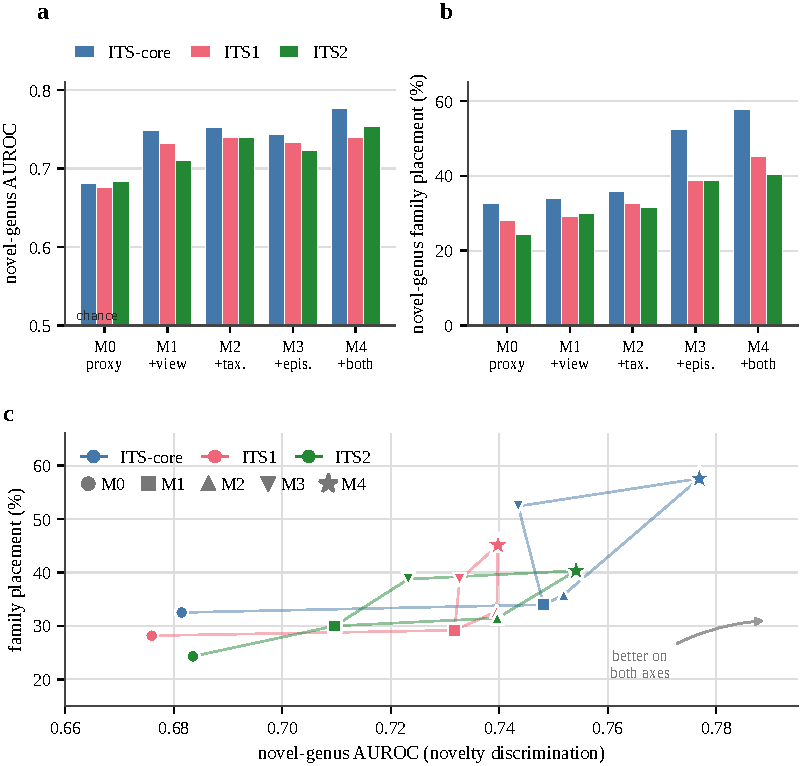
\includegraphics[width=\linewidth]{figures/fig2_ladder.pdf}
\caption{Development ladder, exact-length inference. (a) Novel-genus AUROC, axis
truncated at chance. (b) Novel-genus family placement. (c) The two plotted
against each other. Colour is the barcode view and marker shape the model.}
\label{fig:ladder}
\end{figure}

\begin{table}[htbp]\centering
\begin{threeparttable}
\caption{M4 development retrieval matrix. Every query view was searched against every reference view. Diagonal cells are same-view retrieval; off-diagonal cells measure how far the shared space transfers. Same-view cells in bold.}
\label{tab:m4matrix}
\begin{tabular}{llccc}
\toprule
 & & \multicolumn{3}{c}{reference view} \\
\cmidrule(l){3-5}
metric & query view & ITS-core & ITS1 & ITS2 \\
\midrule
novelty AUROC & ITS-core & \textbf{0.777} & 0.598 & 0.615 \\
 & ITS1 & 0.581 & \textbf{0.740} & 0.490 \\
 & ITS2 & 0.616 & 0.471 & \textbf{0.754} \\
\addlinespace
known-genus NN accuracy & ITS-core & \textbf{69.8\%} & 37.0\% & 27.5\% \\
 & ITS1 & 32.9\% & \textbf{61.8\%} & 2.8\% \\
 & ITS2 & 24.2\% & 3.3\% & \textbf{61.7\%} \\
\addlinespace
novel-genus family NN & ITS-core & \textbf{57.6\%} & 36.3\% & 30.1\% \\
 & ITS1 & 30.0\% & \textbf{45.1\%} & 9.0\% \\
 & ITS2 & 20.6\% & 6.3\% & \textbf{40.3\%} \\
\bottomrule
\end{tabular}
\begin{tablenotes}\footnotesize
\item ITS-core is the strongest bridge to both spacers. Direct ITS1$\leftrightarrow$ITS2 retrieval remains near chance in AUROC and below 7\% in known-genus accuracy, consistent with incomplete alignment of the two spacer-specific representations.
\item Chance for a nearest-neighbour genus assignment over the 4,231 represented genera is approximately 0.02\%, so the spacer-to-spacer cells are weak rather than empty.
\end{tablenotes}
\end{threeparttable}
\end{table}


\begin{figure}[htbp]\centering
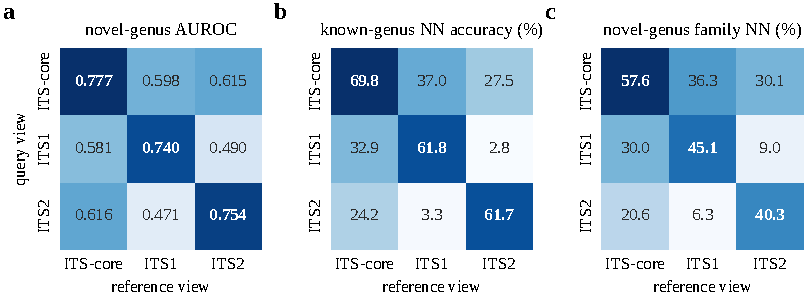
\includegraphics[width=\linewidth]{figures/fig3_crossview_matrix.pdf}
\caption{M4 development retrieval for every query and reference view,
exact-length inference: (a) novel-genus AUROC, (b) known-genus nearest-neighbour
accuracy, (c) novel-genus family placement.}
\label{fig:crossview}
\end{figure}


\section{Historical benchmark}
\label{app:historical}
Identity from the exhaustive, coverage-filtered search and cosine from
exact-length inference on the leakage-safe checkpoint. The sealed values are
deposited as \texttt{data/historical\_benchmark\_sealed.csv}.

\begin{table}[htbp]\centering
\begin{threeparttable}
\caption{Leakage-controlled historical ITS2 benchmark. Percent identity and leakage-safe M4 cosine are scored on identical queries, identical reference collections and an identical conformal procedure, so the comparison is paired throughout. Higher is better except for false novelty, where the target is the nominal $\alpha$.}
\label{tab:historical}
\begin{tabular}{lccc}
\toprule
metric & percent identity & M4 cosine & difference \\
\midrule
AUROC & \textbf{0.768} & 0.703 & +0.065 \\
novel detected, $\alpha=0.01$ & \textbf{14.9\%} & 2.4\% & +12.5 pp \\
novel detected, $\alpha=0.05$ & \textbf{28.1\%} & 11.2\% & +17.0 pp \\
novel detected, $\alpha=0.10$ & \textbf{38.5\%} & 20.9\% & +17.6 pp \\
novel detected, $\alpha=0.20$ & \textbf{54.0\%} & 41.0\% & +13.0 pp \\
false novelty, $\alpha=0.05$ & 4.3\% & 3.9\% & +0.4 pp \\
\addlinespace
family recovery, known species (LSO) & \textbf{91.4\%} & 72.2\% & +19.2 pp \\
family recovery, novel genus (LGO) & \textbf{52.6\%} & 28.2\% & +24.4 pp \\
\bottomrule
\end{tabular}
\begin{tablenotes}\footnotesize
\item $n=1{,}632$ calibration knowns, $1{,}632$ test knowns and 4,444 novel-genus queries, identical for both scores.
\item The AUROC difference is $+0.065$ (95\% CI $+0.046$ to $+0.085$, 10{,}000 paired bootstrap resamples clustered on query genus in both classes). The DeLong test on the same contrast gives $z=11.9$, $p<10^{-16}$; it assumes within-class independence, which the LGO design violates, so the clustered interval is the one to read. Clustering widens the interval by $1.8\times$. McNemar on the $\alpha=0.05$ flag sets separates power from calibration: among novel queries, 872 were flagged by identity alone against 117 by cosine alone ($p<10^{-16}$), while the observed false-novelty rates differ by $0.4$ percentage points.
\item 619 of the 4,444 LGO queries (13.9\%) returned no VSEARCH hit at identity $\geq0.5$ and query coverage $\geq0.8$ and carry the censoring value, against 542 under the default-settings search. All are flagged at $\alpha=0.05$: of the 1,251 novel queries identity flags there, 619 (49\%) are censored rather than scored, so about half of identity's detections on this benchmark are queries with no alignable reference.
\item The M4 cosine column comes from the leakage-safe retraining, fitted to 11\% fewer records and 483 fewer genera than primary M4. DEV was not reopened for that run, so the cost of the mask to model quality is unmeasured.
\item The calibration and test halves of the LSO set are drawn by \texttt{np.random.default\_rng(0).permutation}. Across ten halvings (seeds 0 to 9) the identity advantage ranged from $+0.063$ to $+0.075$ AUROC and every genus-clustered interval excluded zero; seed 0, reported here, lies near the low end. The operating points should therefore be read as approximate.
\item The currently deposited splitter yields 3,264 LSO queries rather than the 3,170 of the earlier novelty manuscript; the LGO count reproduces exactly. These results are therefore a paired comparison on the currently reproducible harness, not a numerical reproduction of the earlier LSO run.
\end{tablenotes}
\end{threeparttable}
\end{table}


\begin{figure}[htbp]\centering
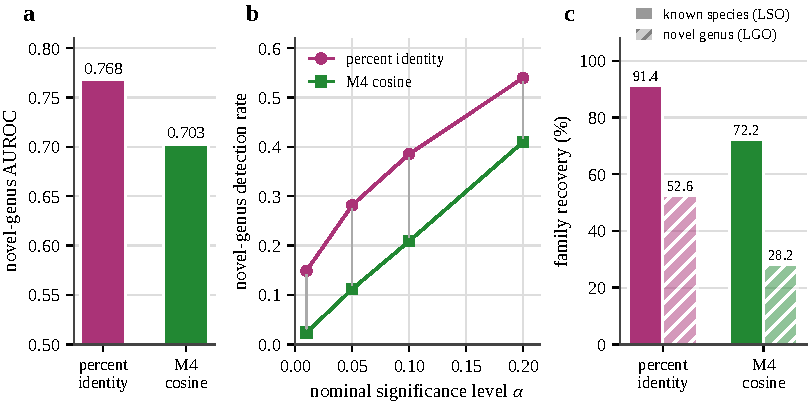
\includegraphics[width=\linewidth]{figures/fig6_historical_identity_vs_cosine.pdf}
\caption{Historical ITS2 benchmark: exhaustive, coverage-filtered identity
against leakage-safe M4 cosine with exact-length inference. (a) Novel-genus AUROC. (b) Detection across conformal
levels. (c) Family recovery.}
\label{fig:historical}
\end{figure}
% flush the appendix floats so none lands among the references
\clearpage
\begin{thebibliography}{99}

\bibitem{angelopoulos2023conformal}
Angelopoulos, A.N., Bates, S. (2023). Conformal prediction: a gentle
introduction. \emph{Foundations and Trends in Machine Learning} 16(4), 494--591.
doi:10.1561/2200000101

\bibitem{badirli2021zeroshot}
Badirli, S., Akata, Z., Mohler, G., Picard, C., Dundar, M.M. (2021). Fine-grained
zero-shot learning with DNA as side information. In \emph{Advances in Neural
Information Processing Systems} 34, 19352--19362.

\bibitem{badirli2023classifying}
Badirli, S., Picard, C.J., Mohler, G., Richert, F., Akata, Z., Dundar, M. (2023).
Classifying the unknown: insect identification with deep hierarchical Bayesian
learning. \emph{Methods in Ecology and Evolution} 14(6), 1515--1530.
doi:10.1111/2041-210X.14104

\bibitem{bengtsson2013itsx}
Bengtsson-Palme, J., Ryberg, M., Hartmann, M., et al. (2013). Improved software
detection and extraction of ITS1 and ITS2 from ribosomal ITS sequences of fungi
and other eukaryotes for analysis of environmental sequencing data.
\emph{Methods in Ecology and Evolution} 4(10), 914--919.
doi:10.1111/2041-210X.12073

\bibitem{fujisawa2026ood}
Fujisawa, T., Imai, T. (2026). Performance and limitations of out-of-distribution
detection for insect DNA barcoding. \emph{Ecology and Evolution}.
doi:10.1002/ece3.73112

\bibitem{hendrycks2017baseline}
Hendrycks, D., Gimpel, K. (2017). A baseline for detecting misclassified and
out-of-distribution examples in neural networks. In \emph{International
Conference on Learning Representations}. arXiv:1610.02136.

\bibitem{ji2021dnabert}
Ji, Y., Zhou, Z., Liu, H., Davuluri, R.V. (2021). DNABERT: pre-trained
bidirectional encoder representations from transformers model for DNA-language
in genome. \emph{Bioinformatics} 37(15), 2112--2120.
doi:10.1093/bioinformatics/btab083

\bibitem{khosla2020supcon}
Khosla, P., Teterwak, P., Wang, C., Sarna, A., Tian, Y., Isola, P.,
Maschinot, A., Liu, C., Krishnan, D. (2020). Supervised contrastive learning. In
\emph{Advances in Neural Information Processing Systems} 33, 18661--18673.

\bibitem{nilsson2019unite}
Nilsson, R.H., Larsson, K.-H., Taylor, A.F.S., et al. (2019). The UNITE database
for molecular identification of fungi: handling dark taxa and parallel taxonomic
classifications. \emph{Nucleic Acids Research} 47(D1), D259--D264.
doi:10.1093/nar/gky1022

\bibitem{obrien2026flag}
O'Brien, A., Mar\'in, C., Parada, P. (2026). A calibrated novelty flag for fungal
ITS metabarcoding: choosing the error rate at which sequences are declared new.
\emph{bioRxiv} 2026.07.29.741524. doi:10.64898/2026.07.29.741524

\bibitem{obrien2026classifiers}
O'Brien, A., Mar\'in, C., Parada, P. (2026). Pretrained deep-learning ITS
classifiers read the flanking regions, not the ITS2 barcode, and so fail on the
amplicon that environmental fungal surveys sequence. \emph{bioRxiv}
2026.07.29.741510. doi:10.64898/2026.07.29.741510

\bibitem{oord2018cpc}
van den Oord, A., Li, Y., Vinyals, O. (2018). Representation learning with
contrastive predictive coding. \emph{arXiv} 1807.03748.

\bibitem{romeijn2024mycoai}
Romeijn, L., Bernatavicius, A., Vu, D. (2024). MycoAI: fast and accurate
taxonomic classification for fungal ITS sequences. \emph{Molecular Ecology
Resources} 24(8), e14006. doi:10.1111/1755-0998.14006

\bibitem{rognes2016vsearch}
Rognes, T., Flouri, T., Nichols, B., Quince, C., Mah\'e, F. (2016). VSEARCH: a
versatile open source tool for metagenomics. \emph{PeerJ} 4, e2584.
doi:10.7717/peerj.2584

\bibitem{snell2017protonet}
Snell, J., Swersky, K., Zemel, R. (2017). Prototypical networks for few-shot
learning. In \emph{Advances in Neural Information Processing Systems} 30,
4077--4087.

\bibitem{sun2022knnood}
Sun, Y., Ming, Y., Zhu, X., Li, Y. (2022). Out-of-distribution detection with
deep nearest neighbors. In \emph{Proceedings of the 39th International
Conference on Machine Learning}, PMLR 162, 20827--20840.

\bibitem{unite2025release}
Abarenkov, K., Zirk, A., Piirmann, T., P\"oh\"onen, R., Ivanov, F., Nilsson,
R.H., K\~oljalg, U. (2025). UNITE general FASTA release for Fungi. Version
19.02.2025. UNITE Community. doi:10.15156/BIO/3301229

\bibitem{vaze2022osr}
Vaze, S., Han, K., Vedaldi, A., Zisserman, A. (2022). Open-set recognition: a
good closed-set classifier is all you need? In \emph{International Conference on
Learning Representations}.

\bibitem{vovk2005}
Vovk, V., Gammerman, A., Shafer, G. (2005). \emph{Algorithmic Learning in a
Random World}. Springer.

\bibitem{wang2007rdp}
Wang, Q., Garrity, G.M., Tiedje, J.M., Cole, J.R. (2007). Naive Bayesian
classifier for rapid assignment of rRNA sequences into the new bacterial
taxonomy. \emph{Applied and Environmental Microbiology} 73(16), 5261--5267.
doi:10.1128/AEM.00062-07


\bibitem{abarenkov2018protax}
Abarenkov, K., Somervuo, P., Nilsson, R.H., Kirk, P.M., Huotari, T., Abrego, N.,
Ovaskainen, O. (2018). PROTAX-fungi: a web-based tool for probabilistic taxonomic
placement of fungal internal transcribed spacer sequences. \emph{New Phytologist}
220(2), 517--525. doi:10.1111/nph.15301

\bibitem{delong1988}
DeLong, E.R., DeLong, D.M., Clarke-Pearson, D.L. (1988). Comparing the areas
under two or more correlated receiver operating characteristic curves: a
nonparametric approach. \emph{Biometrics} 44(3), 837--845.

\bibitem{edgar2016sintax}
Edgar, R.C. (2016). SINTAX: a simple non-Bayesian taxonomy classifier for 16S and
ITS sequences. \emph{bioRxiv}. doi:10.1101/074161

\bibitem{edgar2018accuracy}
Edgar, R.C. (2018). Accuracy of taxonomy prediction for 16S rRNA and fungal ITS
sequences. \emph{PeerJ} 6, e4652. doi:10.7717/peerj.4652

\bibitem{orsholm2026unseen}
Orsholm, J., Zito, A., Somervuo, P., Harrison, J.P., Koskela, M., Ovaskainen, O.,
Braga, M.P., Chazot, N., Roslin, T., Furneaux, B. (2026). Discovering the unseen:
a performance comparison of taxonomic classification methods for unknown DNA
barcodes. \emph{Methods in Ecology and Evolution}. doi:10.1111/2041-210x.70358

\bibitem{zito2023bayesant}
Zito, A., Rigon, T., Dunson, D.B. (2023). Inferring taxonomic placement from DNA
barcoding aiding in discovery of new taxa. \emph{Methods in Ecology and
Evolution} 14(2), 529--542. doi:10.1111/2041-210X.14009

\end{thebibliography}
\end{document}
